\documentclass[1p]{elsarticle_modified}
%\bibliographystyle{elsarticle-num}

%\usepackage[colorlinks]{hyperref}
%\usepackage{abbrmath_seonhwa} %\Abb, \Ascr, \Acal ,\Abf, \Afrak
\usepackage{amsfonts}
\usepackage{amssymb}
\usepackage{amsmath}
\usepackage{amsthm}
\usepackage{scalefnt}
\usepackage{amsbsy}
\usepackage{kotex}
\usepackage{caption}
\usepackage{subfig}
\usepackage{color}
\usepackage{graphicx}
\usepackage{xcolor} %% white, black, red, green, blue, cyan, magenta, yellow
\usepackage{float}
\usepackage{setspace}
\usepackage{hyperref}

\usepackage{tikz}
\usetikzlibrary{arrows}

\usepackage{multirow}
\usepackage{array} % fixed length table
\usepackage{hhline}

%%%%%%%%%%%%%%%%%%%%%
\makeatletter
\renewcommand*\env@matrix[1][\arraystretch]{%
	\edef\arraystretch{#1}%
	\hskip -\arraycolsep
	\let\@ifnextchar\new@ifnextchar
	\array{*\c@MaxMatrixCols c}}
\makeatother %https://tex.stackexchange.com/questions/14071/how-can-i-increase-the-line-spacing-in-a-matrix
%%%%%%%%%%%%%%%

\usepackage[normalem]{ulem}

\newcommand{\msout}[1]{\ifmmode\text{\sout{\ensuremath{#1}}}\else\sout{#1}\fi}
%SOURCE: \msout is \stkout macro in https://tex.stackexchange.com/questions/20609/strikeout-in-math-mode

\newcommand{\cancel}[1]{
	\ifmmode
	{\color{red}\msout{#1}}
	\else
	{\color{red}\sout{#1}}
	\fi
}

\newcommand{\add}[1]{
	{\color{blue}\uwave{#1}}
}

\newcommand{\replace}[2]{
	\ifmmode
	{\color{red}\msout{#1}}{\color{blue}\uwave{#2}}
	\else
	{\color{red}\sout{#1}}{\color{blue}\uwave{#2}}
	\fi
}

\newcommand{\Sol}{\mathcal{S}} %segment
\newcommand{\D}{D} %diagram
\newcommand{\A}{\mathcal{A}} %arc


%%%%%%%%%%%%%%%%%%%%%%%%%%%%%5 test

\def\sl{\operatorname{\textup{SL}}(2,\Cbb)}
\def\psl{\operatorname{\textup{PSL}}(2,\Cbb)}
\def\quan{\mkern 1mu \triangleright \mkern 1mu}

\theoremstyle{definition}
\newtheorem{thm}{Theorem}[section]
\newtheorem{prop}[thm]{Proposition}
\newtheorem{lem}[thm]{Lemma}
\newtheorem{ques}[thm]{Question}
\newtheorem{cor}[thm]{Corollary}
\newtheorem{defn}[thm]{Definition}
\newtheorem{exam}[thm]{Example}
\newtheorem{rmk}[thm]{Remark}
\newtheorem{alg}[thm]{Algorithm}

\newcommand{\I}{\sqrt{-1}}
\begin{document}

%\begin{frontmatter}
%
%\title{Boundary parabolic representations of knots up to 8 crossings}
%
%%% Group authors per affiliation:
%\author{Yunhi Cho} 
%\address{Department of Mathematics, University of Seoul, Seoul, Korea}
%\ead{yhcho@uos.ac.kr}
%
%
%\author{Seonhwa Kim} %\fnref{s_kim}}
%\address{Center for Geometry and Physics, Institute for Basic Science, Pohang, 37673, Korea}
%\ead{ryeona17@ibs.re.kr}
%
%\author{Hyuk Kim}
%\address{Department of Mathematical Sciences, Seoul National University, Seoul 08826, Korea}
%\ead{hyukkim@snu.ac.kr}
%
%\author{Seokbeom Yoon}
%\address{Department of Mathematical Sciences, Seoul National University, Seoul, 08826,  Korea}
%\ead{sbyoon15@snu.ac.kr}
%
%\begin{abstract}
%We find all boundary parabolic representation of knots up to 8 crossings.
%
%\end{abstract}
%\begin{keyword}
%    \MSC[2010] 57M25 
%\end{keyword}
%
%\end{frontmatter}

%\linenumbers
%\tableofcontents
%
\newcommand\colored[1]{\textcolor{white}{\rule[-0.35ex]{0.8em}{1.4ex}}\kern-0.8em\color{red} #1}%
%\newcommand\colored[1]{\textcolor{white}{ #1}\kern-2.17ex	\textcolor{white}{ #1}\kern-1.81ex	\textcolor{white}{ #1}\kern-2.15ex\color{red}#1	}

{\Large $\underline{12a_{0117}~(K12a_{0117})}$}

\setlength{\tabcolsep}{10pt}
\renewcommand{\arraystretch}{1.6}
\vspace{1cm}\begin{tabular}{m{100pt}>{\centering\arraybackslash}m{274pt}}
\multirow{5}{120pt}{
	\centering
	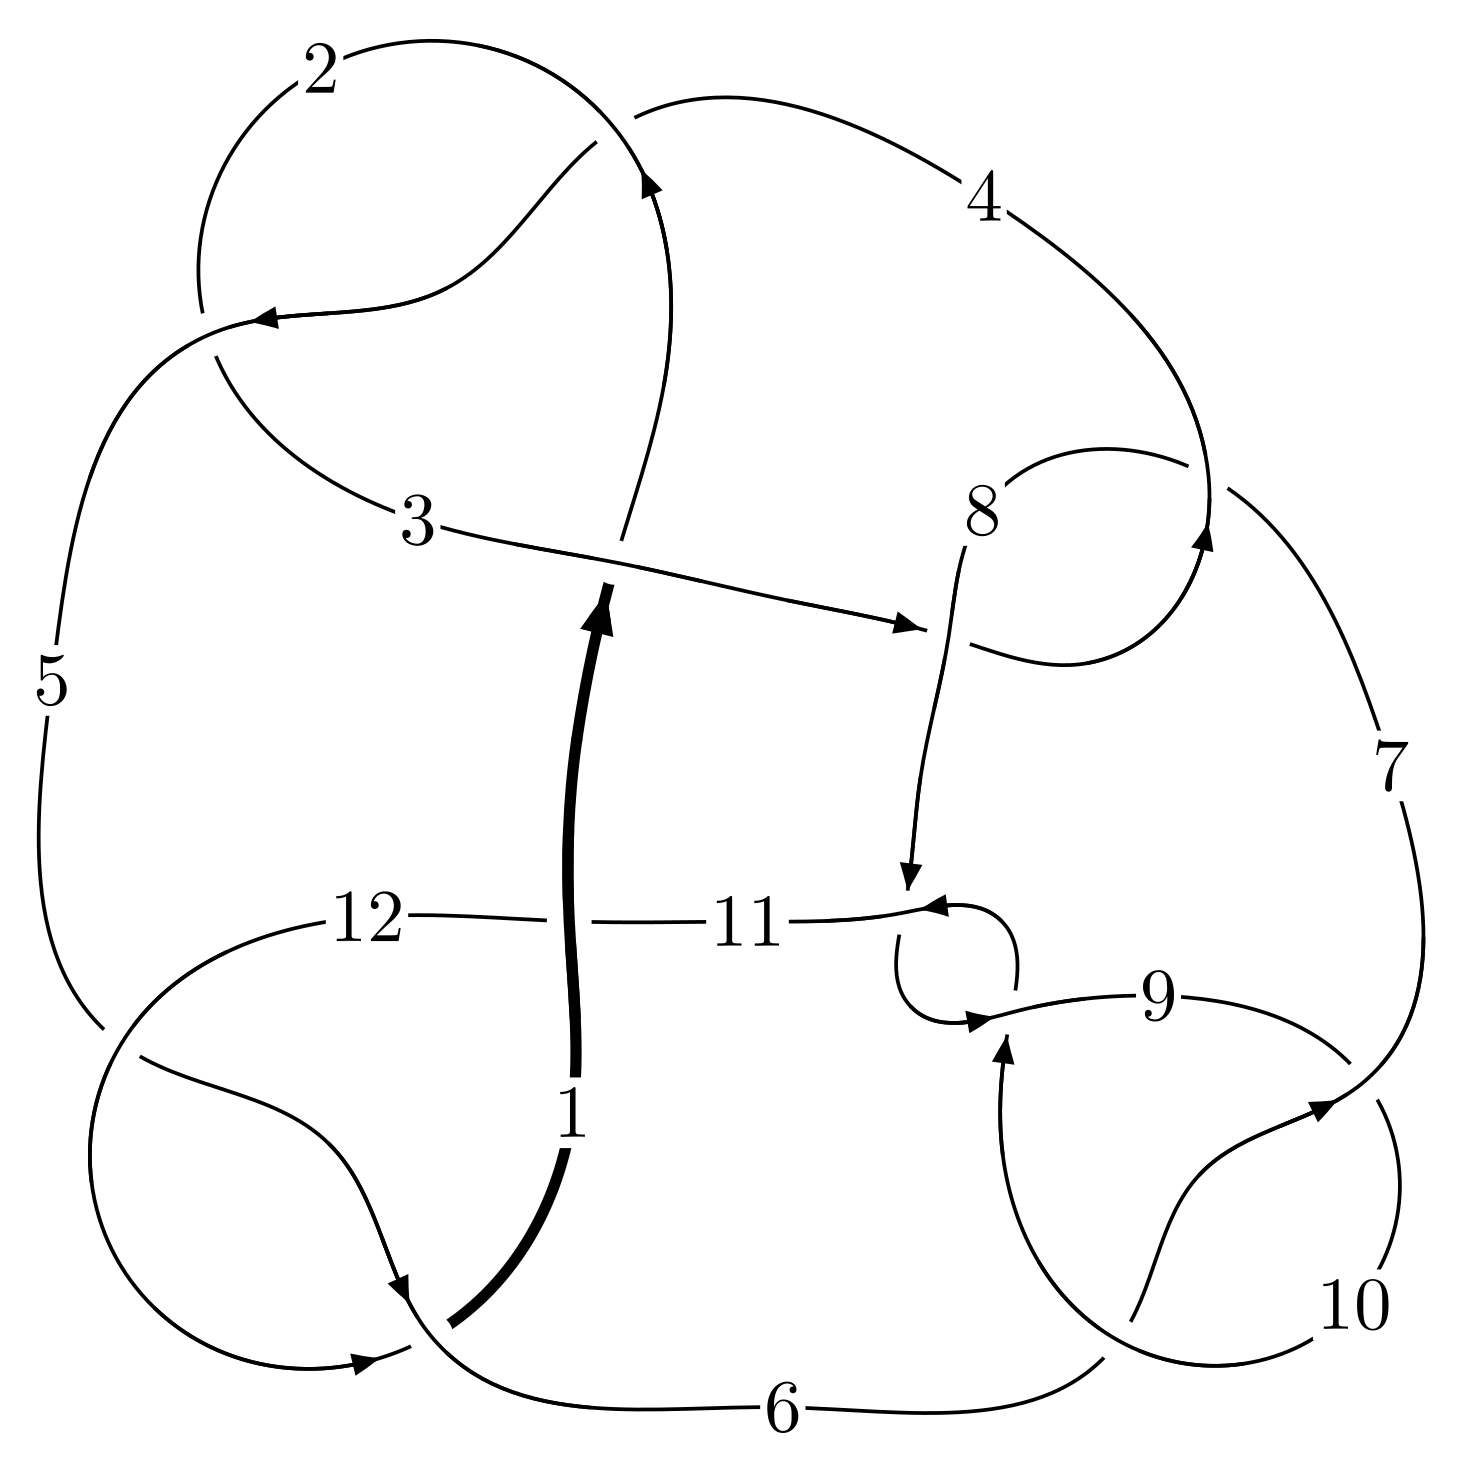
\includegraphics[width=112pt]{../../../GIT/diagram.site/Diagrams/png/918_12a_0117.png}\\
\ \ \ A knot diagram\footnotemark}&
\allowdisplaybreaks
\textbf{Linearized knot diagam} \\
\cline{2-2}
 &
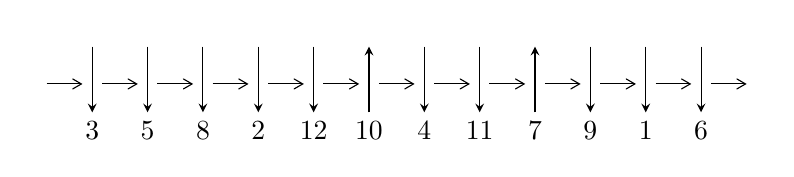
\begin{tikzpicture}[x=20pt, y=17pt]
	% nodes
	\node (C0) at (0, 0) {};
	\node (C1) at (1, 0) {};
	\node (C1U) at (1, +1) {};
	\node (C1D) at (1, -1) {3};

	\node (C2) at (2, 0) {};
	\node (C2U) at (2, +1) {};
	\node (C2D) at (2, -1) {5};

	\node (C3) at (3, 0) {};
	\node (C3U) at (3, +1) {};
	\node (C3D) at (3, -1) {8};

	\node (C4) at (4, 0) {};
	\node (C4U) at (4, +1) {};
	\node (C4D) at (4, -1) {2};

	\node (C5) at (5, 0) {};
	\node (C5U) at (5, +1) {};
	\node (C5D) at (5, -1) {12};

	\node (C6) at (6, 0) {};
	\node (C6U) at (6, +1) {};
	\node (C6D) at (6, -1) {10};

	\node (C7) at (7, 0) {};
	\node (C7U) at (7, +1) {};
	\node (C7D) at (7, -1) {4};

	\node (C8) at (8, 0) {};
	\node (C8U) at (8, +1) {};
	\node (C8D) at (8, -1) {11};

	\node (C9) at (9, 0) {};
	\node (C9U) at (9, +1) {};
	\node (C9D) at (9, -1) {7};

	\node (C10) at (10, 0) {};
	\node (C10U) at (10, +1) {};
	\node (C10D) at (10, -1) {9};

	\node (C11) at (11, 0) {};
	\node (C11U) at (11, +1) {};
	\node (C11D) at (11, -1) {1};

	\node (C12) at (12, 0) {};
	\node (C12U) at (12, +1) {};
	\node (C12D) at (12, -1) {6};
	\node (C13) at (13, 0) {};

	% arrows
	\draw[->,>={angle 60}]
	(C0) edge (C1) (C1) edge (C2) (C2) edge (C3) (C3) edge (C4) (C4) edge (C5) (C5) edge (C6) (C6) edge (C7) (C7) edge (C8) (C8) edge (C9) (C9) edge (C10) (C10) edge (C11) (C11) edge (C12) (C12) edge (C13) ;	\draw[->,>=stealth]
	(C1U) edge (C1D) (C2U) edge (C2D) (C3U) edge (C3D) (C4U) edge (C4D) (C5U) edge (C5D) (C6D) edge (C6U) (C7U) edge (C7D) (C8U) edge (C8D) (C9D) edge (C9U) (C10U) edge (C10D) (C11U) edge (C11D) (C12U) edge (C12D) ;
	\end{tikzpicture} \\
\hhline{~~} \\& 
\textbf{Solving Sequence} \\ \cline{2-2} 
 &
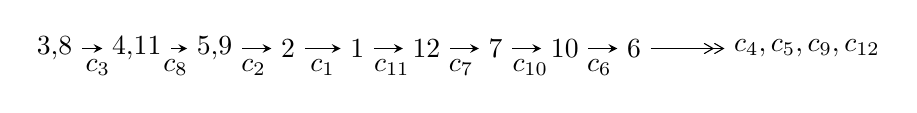
\begin{tikzpicture}[x=25pt, y=7pt]
	% node
	\node (A0) at (-1/8, 0) {3,8};
	\node (A1) at (17/16, 0) {4,11};
	\node (A2) at (35/16, 0) {5,9};
	\node (A3) at (13/4, 0) {2};
	\node (A4) at (17/4, 0) {1};
	\node (A5) at (21/4, 0) {12};
	\node (A6) at (25/4, 0) {7};
	\node (A7) at (29/4, 0) {10};
	\node (A8) at (33/4, 0) {6};
	\node (C1) at (1/2, -1) {$c_{3}$};
	\node (C2) at (13/8, -1) {$c_{8}$};
	\node (C3) at (11/4, -1) {$c_{2}$};
	\node (C4) at (15/4, -1) {$c_{1}$};
	\node (C5) at (19/4, -1) {$c_{11}$};
	\node (C6) at (23/4, -1) {$c_{7}$};
	\node (C7) at (27/4, -1) {$c_{10}$};
	\node (C8) at (31/4, -1) {$c_{6}$};
	\node (A9) at (43/4, 0) {$c_{4},c_{5},c_{9},c_{12}$};

	% edge
	\draw[->,>=stealth]	
	(A0) edge (A1) (A1) edge (A2) (A2) edge (A3) (A3) edge (A4) (A4) edge (A5) (A5) edge (A6) (A6) edge (A7) (A7) edge (A8) ;
	\draw[->>,>={angle 60}]	
	(A8) edge (A9);
\end{tikzpicture} \\ 

\end{tabular} \\

\footnotetext{
The image of knot diagram is generated by the software ``\textbf{Draw programme}" developed by Andrew Bartholomew(\url{http://www.layer8.co.uk/maths/draw/index.htm\#Running-draw}), where we modified some parts for our purpose(\url{https://github.com/CATsTAILs/LinksPainter}).
}\phantom \\ \newline 
\centering \textbf{Ideals for irreducible components\footnotemark of $X_{\text{par}}$} 
 
\begin{align*}
I^u_{1}&=\langle 
3.99437\times10^{56} u^{42}-1.17694\times10^{57} u^{41}+\cdots+1.61592\times10^{58} d+3.40126\times10^{57},\\
\phantom{I^u_{1}}&\phantom{= \langle  }3.31530\times10^{55} u^{42}-3.28100\times10^{56} u^{41}+\cdots+3.23183\times10^{58} c+4.23971\times10^{58},\\
\phantom{I^u_{1}}&\phantom{= \langle  }-4.23475\times10^{55} u^{42}+5.01357\times10^{55} u^{41}+\cdots+1.61592\times10^{58} b-1.64157\times10^{57},\\
\phantom{I^u_{1}}&\phantom{= \langle  }1.77513\times10^{55} u^{42}-8.50273\times10^{55} u^{41}+\cdots+3.23183\times10^{58} a-3.36911\times10^{58},\;u^{43}-3 u^{42}+\cdots+64 u-32\rangle \\
I^u_{2}&=\langle 
5.02544\times10^{17} u^{34}-6.24095\times10^{17} u^{33}+\cdots+3.02602\times10^{18} d+2.19741\times10^{18},\\
\phantom{I^u_{2}}&\phantom{= \langle  }-6.42534\times10^{19} u^{34}-3.74850\times10^{19} u^{33}+\cdots+4.84163\times10^{19} c+2.56918\times10^{19},\\
\phantom{I^u_{2}}&\phantom{= \langle  }4.96996\times10^{18} a u^{34}-6.75491\times10^{18} u^{34}+\cdots-1.88128\times10^{19} a-4.81090\times10^{19},\\
\phantom{I^u_{2}}&\phantom{= \langle  }-5.09108\times10^{19} a u^{34}-2.42015\times10^{19} u^{34}+\cdots-1.99866\times10^{19} a-6.67500\times10^{19},\;u^{35}+u^{34}+\cdots-8 u-4\rangle \\
\\
I^v_{1}&=\langle 
c,\;d+1,\;b,\;a-1,\;v^2+v+1\rangle \\
I^v_{2}&=\langle 
a,\;d+1,\;c+a,\;b-1,\;v^2+v+1\rangle \\
I^v_{3}&=\langle 
a,\;d,\;c+1,\;b-1,\;v+1\rangle \\
I^v_{4}&=\langle 
a,\;d^2 v^2- d v+1,\;v^2 d c- v^2 d- c v+a+v,\;d a- c+1,\;c^2 v^2- c a v-2 v^2 c+a^2+a v+v^2,\;b-1\rangle \\
\end{align*}
\raggedright * 5 irreducible components of $\dim_{\mathbb{C}}=0$, with total 118 representations.\\
\raggedright * 1 irreducible components of $\dim_{\mathbb{C}}=1$ \\
\footnotetext{All coefficients of polynomials are rational numbers. But the coefficients are sometimes approximated in decimal forms when there is not enough margin.}
\newpage
\renewcommand{\arraystretch}{1}
\centering \section*{I. $I^u_{1}= \langle 3.99\times10^{56} u^{42}-1.18\times10^{57} u^{41}+\cdots+1.62\times10^{58} d+3.40\times10^{57},\;3.32\times10^{55} u^{42}-3.28\times10^{56} u^{41}+\cdots+3.23\times10^{58} c+4.24\times10^{58},\;-4.23\times10^{55} u^{42}+5.01\times10^{55} u^{41}+\cdots+1.62\times10^{58} b-1.64\times10^{57},\;1.78\times10^{55} u^{42}-8.50\times10^{55} u^{41}+\cdots+3.23\times10^{58} a-3.37\times10^{58},\;u^{43}-3 u^{42}+\cdots+64 u-32 \rangle$}
\flushleft \textbf{(i) Arc colorings}\\
\begin{tabular}{m{7pt} m{180pt} m{7pt} m{180pt} }
\flushright $a_{3}=$&$\begin{pmatrix}1\\0\end{pmatrix}$ \\
\flushright $a_{8}=$&$\begin{pmatrix}0\\u\end{pmatrix}$ \\
\flushright $a_{4}=$&$\begin{pmatrix}1\\u^2\end{pmatrix}$ \\
\flushright $a_{11}=$&$\begin{pmatrix}-0.00102583 u^{42}+0.0101521 u^{41}+\cdots-0.345721 u-1.31186\\-0.0247189 u^{42}+0.0728342 u^{41}+\cdots-0.100365 u-0.210485\end{pmatrix}$ \\
\flushright $a_{5}=$&$\begin{pmatrix}-0.000549265 u^{42}+0.00263093 u^{41}+\cdots+0.260997 u+1.04248\\0.00262065 u^{42}-0.00310262 u^{41}+\cdots-0.582583 u+0.101587\end{pmatrix}$ \\
\flushright $a_{9}=$&$\begin{pmatrix}0.0176645 u^{42}-0.0450742 u^{41}+\cdots-2.28416 u-0.505300\\-0.0151840 u^{42}+0.0606156 u^{41}+\cdots+2.05478 u-1.00258\end{pmatrix}$ \\
\flushright $a_{2}=$&$\begin{pmatrix}-0.000549265 u^{42}+0.00263093 u^{41}+\cdots+0.260997 u+1.04248\\-0.00664203 u^{42}+0.00629753 u^{41}+\cdots+0.502086 u-0.0701269\end{pmatrix}$ \\
\flushright $a_{1}=$&$\begin{pmatrix}-0.00719130 u^{42}+0.00892846 u^{41}+\cdots+0.763083 u+0.972348\\-0.00664203 u^{42}+0.00629753 u^{41}+\cdots+0.502086 u-0.0701269\end{pmatrix}$ \\
\flushright $a_{12}=$&$\begin{pmatrix}-0.00209131 u^{42}+0.0152778 u^{41}+\cdots-0.305485 u-1.53809\\-0.0237130 u^{42}+0.0774882 u^{41}+\cdots-0.381714 u-0.292656\end{pmatrix}$ \\
\flushright $a_{7}=$&$\begin{pmatrix}u\\u^3+u\end{pmatrix}$ \\
\flushright $a_{10}=$&$\begin{pmatrix}0.0268260 u^{42}-0.0643618 u^{41}+\cdots-3.05990 u-0.696376\\0.000919890 u^{42}+0.0297984 u^{41}+\cdots+1.04761 u-0.931356\end{pmatrix}$ \\
\flushright $a_{6}=$&$\begin{pmatrix}-0.0236931 u^{42}+0.0626821 u^{41}+\cdots+0.245356 u+1.10137\\-0.0252351 u^{42}+0.0753290 u^{41}+\cdots-0.321126 u-0.479194\end{pmatrix}$\\&\end{tabular}
\flushleft \textbf{(ii) Obstruction class $= -1$}\\~\\
\flushleft \textbf{(iii) Cusp Shapes $= -0.141642 u^{42}+0.373966 u^{41}+\cdots+18.4912 u-10.3634$}\\~\\
\newpage\renewcommand{\arraystretch}{1}
\flushleft \textbf{(iv) u-Polynomials at the component}\newline \\
\begin{tabular}{m{50pt}|m{274pt}}
Crossings & \hspace{64pt}u-Polynomials at each crossing \\
\hline $$\begin{aligned}c_{1},c_{11}\end{aligned}$$&$\begin{aligned}
&u^{43}+19 u^{42}+\cdots+11 u+1
\end{aligned}$\\
\hline $$\begin{aligned}c_{2},c_{4},c_{5}\\c_{12}\end{aligned}$$&$\begin{aligned}
&u^{43}-5 u^{42}+\cdots-5 u+1
\end{aligned}$\\
\hline $$\begin{aligned}c_{3},c_{7}\end{aligned}$$&$\begin{aligned}
&u^{43}+3 u^{42}+\cdots+64 u+32
\end{aligned}$\\
\hline $$\begin{aligned}c_{6},c_{9}\end{aligned}$$&$\begin{aligned}
&u^{43}+u^{42}+\cdots+8 u+4
\end{aligned}$\\
\hline $$\begin{aligned}c_{8},c_{10}\end{aligned}$$&$\begin{aligned}
&u^{43}+15 u^{42}+\cdots+88 u-16
\end{aligned}$\\
\hline
\end{tabular}\\~\\
\newpage\renewcommand{\arraystretch}{1}
\flushleft \textbf{(v) Riley Polynomials at the component}\newline \\
\begin{tabular}{m{50pt}|m{274pt}}
Crossings & \hspace{64pt}Riley Polynomials at each crossing \\
\hline $$\begin{aligned}c_{1},c_{11}\end{aligned}$$&$\begin{aligned}
&y^{43}+21 y^{42}+\cdots-117 y-1
\end{aligned}$\\
\hline $$\begin{aligned}c_{2},c_{4},c_{5}\\c_{12}\end{aligned}$$&$\begin{aligned}
&y^{43}-19 y^{42}+\cdots+11 y-1
\end{aligned}$\\
\hline $$\begin{aligned}c_{3},c_{7}\end{aligned}$$&$\begin{aligned}
&y^{43}+15 y^{42}+\cdots-1024 y-1024
\end{aligned}$\\
\hline $$\begin{aligned}c_{6},c_{9}\end{aligned}$$&$\begin{aligned}
&y^{43}+15 y^{42}+\cdots+88 y-16
\end{aligned}$\\
\hline $$\begin{aligned}c_{8},c_{10}\end{aligned}$$&$\begin{aligned}
&y^{43}+27 y^{42}+\cdots+18208 y-256
\end{aligned}$\\
\hline
\end{tabular}\\~\\
\newpage\flushleft \textbf{(vi) Complex Volumes and Cusp Shapes}
$$\begin{array}{c|c|c}  
\text{Solutions to }I^u_{1}& \I (\text{vol} + \sqrt{-1}CS) & \text{Cusp shape}\\
 \hline 
\begin{aligned}
u &= -0.083173 + 0.999400 I \\
a &= \phantom{-}0.72843 - 1.47481 I \\
b &= -0.730777 + 0.545079 I \\
c &= \phantom{-}0.847687 + 0.941729 I \\
d &= -0.167389 - 0.931774 I\end{aligned}
 & -0.05445 + 4.88438 I & -6.23953 - 8.26907 I \\ \hline\begin{aligned}
u &= -0.083173 - 0.999400 I \\
a &= \phantom{-}0.72843 + 1.47481 I \\
b &= -0.730777 - 0.545079 I \\
c &= \phantom{-}0.847687 - 0.941729 I \\
d &= -0.167389 + 0.931774 I\end{aligned}
 & -0.05445 - 4.88438 I & -6.23953 + 8.26907 I \\ \hline\begin{aligned}
u &= -0.853926 + 0.430623 I \\
a &= \phantom{-}0.481539 - 0.101502 I \\
b &= \phantom{-}0.988333 + 0.419116 I \\
c &= -0.433251 + 0.229265 I \\
d &= -1.40759 + 0.95521 I\end{aligned}
 & -2.38574 - 3.27178 I & -9.17419 + 4.94523 I \\ \hline\begin{aligned}
u &= -0.853926 - 0.430623 I \\
a &= \phantom{-}0.481539 + 0.101502 I \\
b &= \phantom{-}0.988333 - 0.419116 I \\
c &= -0.433251 - 0.229265 I \\
d &= -1.40759 - 0.95521 I\end{aligned}
 & -2.38574 + 3.27178 I & -9.17419 - 4.94523 I \\ \hline\begin{aligned}
u &= \phantom{-}1.033880 + 0.177916 I \\
a &= \phantom{-}0.555689 - 0.233546 I \\
b &= \phantom{-}0.529415 + 0.642786 I \\
c &= -0.074981 + 1.239350 I \\
d &= -0.257235 + 0.960210 I\end{aligned}
 & \phantom{-}2.18783 + 1.46576 I & -4.39540 + 0.53246 I \\ \hline\begin{aligned}
u &= \phantom{-}1.033880 - 0.177916 I \\
a &= \phantom{-}0.555689 + 0.233546 I \\
b &= \phantom{-}0.529415 - 0.642786 I \\
c &= -0.074981 - 1.239350 I \\
d &= -0.257235 - 0.960210 I\end{aligned}
 & \phantom{-}2.18783 - 1.46576 I & -4.39540 - 0.53246 I\\
 \hline 
 \end{array}$$\newpage$$\begin{array}{c|c|c}  
\text{Solutions to }I^u_{1}& \I (\text{vol} + \sqrt{-1}CS) & \text{Cusp shape}\\
 \hline 
\begin{aligned}
u &= -1.073470 + 0.049653 I \\
a &= \phantom{-}0.530276 + 0.204737 I \\
b &= \phantom{-}0.641163 - 0.633645 I \\
c &= \phantom{-}0.195783 - 1.125570 I \\
d &= -0.132889 - 0.974636 I\end{aligned}
 & \phantom{-}2.38615 + 4.03105 I & -4.49490 - 6.55598 I \\ \hline\begin{aligned}
u &= -1.073470 - 0.049653 I \\
a &= \phantom{-}0.530276 - 0.204737 I \\
b &= \phantom{-}0.641163 + 0.633645 I \\
c &= \phantom{-}0.195783 + 1.125570 I \\
d &= -0.132889 + 0.974636 I\end{aligned}
 & \phantom{-}2.38615 - 4.03105 I & -4.49490 + 6.55598 I \\ \hline\begin{aligned}
u &= -0.118650 + 1.091750 I \\
a &= \phantom{-}0.665477 + 1.093120 I \\
b &= -0.593668 - 0.667444 I \\
c &= \phantom{-}0.042888 - 0.446984 I \\
d &= -0.181308 + 1.017000 I\end{aligned}
 & \phantom{-}3.02575 - 1.21250 I & -0.81942 + 2.86814 I \\ \hline\begin{aligned}
u &= -0.118650 - 1.091750 I \\
a &= \phantom{-}0.665477 - 1.093120 I \\
b &= -0.593668 + 0.667444 I \\
c &= \phantom{-}0.042888 + 0.446984 I \\
d &= -0.181308 - 1.017000 I\end{aligned}
 & \phantom{-}3.02575 + 1.21250 I & -0.81942 - 2.86814 I \\ \hline\begin{aligned}
u &= \phantom{-}0.359241 + 0.820253 I \\
a &= \phantom{-}0.870329 - 0.688965 I \\
b &= -0.293648 + 0.559159 I \\
c &= -0.888721 + 0.717011 I \\
d &= -0.421777 - 0.556156 I\end{aligned}
 & -0.40821 - 1.76300 I & -5.68682 + 2.17312 I \\ \hline\begin{aligned}
u &= \phantom{-}0.359241 - 0.820253 I \\
a &= \phantom{-}0.870329 + 0.688965 I \\
b &= -0.293648 - 0.559159 I \\
c &= -0.888721 - 0.717011 I \\
d &= -0.421777 + 0.556156 I\end{aligned}
 & -0.40821 + 1.76300 I & -5.68682 - 2.17312 I\\
 \hline 
 \end{array}$$\newpage$$\begin{array}{c|c|c}  
\text{Solutions to }I^u_{1}& \I (\text{vol} + \sqrt{-1}CS) & \text{Cusp shape}\\
 \hline 
\begin{aligned}
u &= \phantom{-}0.910628 + 0.648287 I \\
a &= \phantom{-}0.449928 + 0.096871 I \\
b &= \phantom{-}1.124110 - 0.457326 I \\
c &= -0.725195 + 0.750875 I \\
d &= -2.15758 + 0.22862 I\end{aligned}
 & -6.78885 + 5.21532 I & -15.4874 - 4.9651 I \\ \hline\begin{aligned}
u &= \phantom{-}0.910628 - 0.648287 I \\
a &= \phantom{-}0.449928 - 0.096871 I \\
b &= \phantom{-}1.124110 + 0.457326 I \\
c &= -0.725195 - 0.750875 I \\
d &= -2.15758 - 0.22862 I\end{aligned}
 & -6.78885 - 5.21532 I & -15.4874 + 4.9651 I \\ \hline\begin{aligned}
u &= \phantom{-}0.653698 + 0.530431 I \\
a &= \phantom{-}0.474331 + 0.068978 I \\
b &= \phantom{-}1.064570 - 0.300236 I \\
c &= -1.46607 - 0.52025 I \\
d &= -2.88991 - 1.78080 I\end{aligned}
 & -4.07070 - 1.09789 I & -13.44053 + 1.40134 I \\ \hline\begin{aligned}
u &= \phantom{-}0.653698 - 0.530431 I \\
a &= \phantom{-}0.474331 - 0.068978 I \\
b &= \phantom{-}1.064570 + 0.300236 I \\
c &= -1.46607 + 0.52025 I \\
d &= -2.88991 + 1.78080 I\end{aligned}
 & -4.07070 + 1.09789 I & -13.44053 - 1.40134 I \\ \hline\begin{aligned}
u &= \phantom{-}0.576447 + 1.031310 I \\
a &= -0.28667 + 1.83591 I \\
b &= -1.083030 - 0.531725 I \\
c &= \phantom{-}0.534742 + 1.166610 I \\
d &= -1.301930 - 0.329738 I\end{aligned}
 & -2.58520 - 3.71825 I & -9.87585 + 4.37570 I \\ \hline\begin{aligned}
u &= \phantom{-}0.576447 - 1.031310 I \\
a &= -0.28667 - 1.83591 I \\
b &= -1.083030 + 0.531725 I \\
c &= \phantom{-}0.534742 - 1.166610 I \\
d &= -1.301930 + 0.329738 I\end{aligned}
 & -2.58520 + 3.71825 I & -9.87585 - 4.37570 I\\
 \hline 
 \end{array}$$\newpage$$\begin{array}{c|c|c}  
\text{Solutions to }I^u_{1}& \I (\text{vol} + \sqrt{-1}CS) & \text{Cusp shape}\\
 \hline 
\begin{aligned}
u &= -1.098260 + 0.588414 I \\
a &= \phantom{-}0.444497 - 0.121481 I \\
b &= \phantom{-}1.093370 + 0.572119 I \\
c &= \phantom{-}0.249890 - 0.823067 I \\
d &= -1.021840 - 0.591171 I\end{aligned}
 & -0.56681 - 5.57701 I & -7.91552 + 3.90122 I \\ \hline\begin{aligned}
u &= -1.098260 - 0.588414 I \\
a &= \phantom{-}0.444497 + 0.121481 I \\
b &= \phantom{-}1.093370 - 0.572119 I \\
c &= \phantom{-}0.249890 + 0.823067 I \\
d &= -1.021840 + 0.591171 I\end{aligned}
 & -0.56681 + 5.57701 I & -7.91552 - 3.90122 I \\ \hline\begin{aligned}
u &= -0.614898 + 1.118930 I \\
a &= -0.31373 - 1.65536 I \\
b &= -1.110520 + 0.583151 I \\
c &= \phantom{-}0.160557 - 0.564023 I \\
d &= -0.993758 + 0.779989 I\end{aligned}
 & -0.28043 + 8.69625 I & -6.61034 - 7.94559 I \\ \hline\begin{aligned}
u &= -0.614898 - 1.118930 I \\
a &= -0.31373 + 1.65536 I \\
b &= -1.110520 - 0.583151 I \\
c &= \phantom{-}0.160557 + 0.564023 I \\
d &= -0.993758 - 0.779989 I\end{aligned}
 & -0.28043 - 8.69625 I & -6.61034 + 7.94559 I \\ \hline\begin{aligned}
u &= \phantom{-}1.109210 + 0.657844 I \\
a &= \phantom{-}0.436604 + 0.117557 I \\
b &= \phantom{-}1.135580 - 0.575012 I \\
c &= \phantom{-}0.205444 + 1.179480 I \\
d &= -1.16587 + 0.97462 I\end{aligned}
 & -1.67059 + 11.25340 I & -9.77881 - 8.46956 I \\ \hline\begin{aligned}
u &= \phantom{-}1.109210 - 0.657844 I \\
a &= \phantom{-}0.436604 - 0.117557 I \\
b &= \phantom{-}1.135580 + 0.575012 I \\
c &= \phantom{-}0.205444 - 1.179480 I \\
d &= -1.16587 - 0.97462 I\end{aligned}
 & -1.67059 - 11.25340 I & -9.77881 + 8.46956 I\\
 \hline 
 \end{array}$$\newpage$$\begin{array}{c|c|c}  
\text{Solutions to }I^u_{1}& \I (\text{vol} + \sqrt{-1}CS) & \text{Cusp shape}\\
 \hline 
\begin{aligned}
u &= \phantom{-}0.724262 + 1.081360 I \\
a &= -0.51124 + 1.64089 I \\
b &= -1.173080 - 0.555502 I \\
c &= -0.733855 + 0.745817 I \\
d &= -1.52033 - 1.25212 I\end{aligned}
 & -5.40682 - 11.27400 I & -13.1483 + 8.7166 I \\ \hline\begin{aligned}
u &= \phantom{-}0.724262 - 1.081360 I \\
a &= -0.51124 - 1.64089 I \\
b &= -1.173080 + 0.555502 I \\
c &= -0.733855 - 0.745817 I \\
d &= -1.52033 + 1.25212 I\end{aligned}
 & -5.40682 + 11.27400 I & -13.1483 - 8.7166 I \\ \hline\begin{aligned}
u &= -0.460216 + 1.229810 I \\
a &= \phantom{-}0.522317 + 0.781774 I \\
b &= -0.409134 - 0.884374 I \\
c &= -0.886956 + 0.201557 I \\
d &= -0.82278 + 1.35195 I\end{aligned}
 & \phantom{-}6.33622 + 1.07199 I & -1.20689 + 1.13710 I \\ \hline\begin{aligned}
u &= -0.460216 - 1.229810 I \\
a &= \phantom{-}0.522317 - 0.781774 I \\
b &= -0.409134 + 0.884374 I \\
c &= -0.886956 - 0.201557 I \\
d &= -0.82278 - 1.35195 I\end{aligned}
 & \phantom{-}6.33622 - 1.07199 I & -1.20689 - 1.13710 I \\ \hline\begin{aligned}
u &= \phantom{-}0.548223 + 1.211710 I \\
a &= \phantom{-}0.521334 - 0.726495 I \\
b &= -0.347993 + 0.908591 I \\
c &= -1.151280 - 0.142674 I \\
d &= -1.06491 - 1.27360 I\end{aligned}
 & \phantom{-}5.47474 - 6.91618 I & -2.74163 + 4.17963 I \\ \hline\begin{aligned}
u &= \phantom{-}0.548223 - 1.211710 I \\
a &= \phantom{-}0.521334 + 0.726495 I \\
b &= -0.347993 - 0.908591 I \\
c &= -1.151280 + 0.142674 I \\
d &= -1.06491 + 1.27360 I\end{aligned}
 & \phantom{-}5.47474 + 6.91618 I & -2.74163 - 4.17963 I\\
 \hline 
 \end{array}$$\newpage$$\begin{array}{c|c|c}  
\text{Solutions to }I^u_{1}& \I (\text{vol} + \sqrt{-1}CS) & \text{Cusp shape}\\
 \hline 
\begin{aligned}
u &= \phantom{-}0.168268 + 1.366960 I \\
a &= \phantom{-}0.219555 + 1.223470 I \\
b &= -0.857901 - 0.791847 I \\
c &= \phantom{-}0.981919 + 0.112942 I \\
d &= \phantom{-}0.509117 + 0.733224 I\end{aligned}
 & \phantom{-}7.94604 - 2.88039 I & -2.40290 + 2.87135 I \\ \hline\begin{aligned}
u &= \phantom{-}0.168268 - 1.366960 I \\
a &= \phantom{-}0.219555 - 1.223470 I \\
b &= -0.857901 + 0.791847 I \\
c &= \phantom{-}0.981919 - 0.112942 I \\
d &= \phantom{-}0.509117 - 0.733224 I\end{aligned}
 & \phantom{-}7.94604 + 2.88039 I & -2.40290 - 2.87135 I \\ \hline\begin{aligned}
u &= \phantom{-}0.620383\phantom{ +0.000000I} \\
a &= \phantom{-}0.635515\phantom{ +0.000000I} \\
b &= \phantom{-}0.573528\phantom{ +0.000000I} \\
c &= \phantom{-}0.187133\phantom{ +0.000000I} \\
d &= \phantom{-}0.872137\phantom{ +0.000000I}\end{aligned}
 & -1.07886\phantom{ +0.000000I} & -8.06050\phantom{ +0.000000I} \\ \hline\begin{aligned}
u &= -0.256404 + 1.367180 I \\
a &= \phantom{-}0.141032 - 1.272300 I \\
b &= -0.913934 + 0.776435 I \\
c &= \phantom{-}1.080980 - 0.022426 I \\
d &= \phantom{-}0.549850 - 0.430577 I\end{aligned}
 & \phantom{-}7.59831 + 8.92002 I & -3.37196 - 8.11870 I \\ \hline\begin{aligned}
u &= -0.256404 - 1.367180 I \\
a &= \phantom{-}0.141032 + 1.272300 I \\
b &= -0.913934 - 0.776435 I \\
c &= \phantom{-}1.080980 + 0.022426 I \\
d &= \phantom{-}0.549850 + 0.430577 I\end{aligned}
 & \phantom{-}7.59831 - 8.92002 I & -3.37196 + 8.11870 I \\ \hline\begin{aligned}
u &= \phantom{-}0.170237 + 0.574659 I \\
a &= \phantom{-}1.248050 - 0.407611 I \\
b &= -0.275978 + 0.236465 I \\
c &= -1.39991 + 0.71798 I \\
d &= \phantom{-}0.022364 - 0.261910 I\end{aligned}
 & -0.37797 - 1.66748 I & -2.59196 + 2.78569 I\\
 \hline 
 \end{array}$$\newpage$$\begin{array}{c|c|c}  
\text{Solutions to }I^u_{1}& \I (\text{vol} + \sqrt{-1}CS) & \text{Cusp shape}\\
 \hline 
\begin{aligned}
u &= \phantom{-}0.170237 - 0.574659 I \\
a &= \phantom{-}1.248050 + 0.407611 I \\
b &= -0.275978 - 0.236465 I \\
c &= -1.39991 - 0.71798 I \\
d &= \phantom{-}0.022364 + 0.261910 I\end{aligned}
 & -0.37797 + 1.66748 I & -2.59196 - 2.78569 I \\ \hline\begin{aligned}
u &= -0.766704 + 1.185140 I \\
a &= -0.48729 - 1.47075 I \\
b &= -1.202990 + 0.612671 I \\
c &= -0.773518 + 0.191669 I \\
d &= -1.04186 + 1.80633 I\end{aligned}
 & \phantom{-}1.37987 + 12.30340 I & -8.00000 - 6.92563 I \\ \hline\begin{aligned}
u &= -0.766704 - 1.185140 I \\
a &= -0.48729 + 1.47075 I \\
b &= -1.202990 - 0.612671 I \\
c &= -0.773518 - 0.191669 I \\
d &= -1.04186 - 1.80633 I\end{aligned}
 & \phantom{-}1.37987 - 12.30340 I & -8.00000 + 6.92563 I \\ \hline\begin{aligned}
u &= \phantom{-}0.80758 + 1.17123 I \\
a &= -0.54459 + 1.45657 I \\
b &= -1.225210 - 0.602344 I \\
c &= -1.124940 - 0.247998 I \\
d &= -1.24308 - 2.01707 I\end{aligned}
 & \phantom{-}0.0200 - 18.1731 I & -8.00000 + 11.31467 I \\ \hline\begin{aligned}
u &= \phantom{-}0.80758 - 1.17123 I \\
a &= -0.54459 - 1.45657 I \\
b &= -1.225210 + 0.602344 I \\
c &= -1.124940 + 0.247998 I \\
d &= -1.24308 + 2.01707 I\end{aligned}
 & \phantom{-}0.0200 + 18.1731 I & -8.00000 - 11.31467 I \\ \hline\begin{aligned}
u &= -0.546169 + 0.144967 I \\
a &= \phantom{-}0.536373 - 0.039062 I \\
b &= \phantom{-}0.854540 + 0.135059 I \\
c &= \phantom{-}0.76523 + 1.50364 I \\
d &= \phantom{-}1.77463 + 3.06017 I\end{aligned}
 & -2.99504 - 2.52590 I & -15.3721 + 4.9240 I\\
 \hline 
 \end{array}$$\newpage$$\begin{array}{c|c|c}  
\text{Solutions to }I^u_{1}& \I (\text{vol} + \sqrt{-1}CS) & \text{Cusp shape}\\
 \hline 
\begin{aligned}
u &= -0.546169 - 0.144967 I \\
a &= \phantom{-}0.536373 + 0.039062 I \\
b &= \phantom{-}0.854540 - 0.135059 I \\
c &= \phantom{-}0.76523 - 1.50364 I \\
d &= \phantom{-}1.77463 - 3.06017 I\end{aligned}
 & -2.99504 + 2.52590 I & -15.3721 - 4.9240 I\\
 \hline 
 \end{array}$$\newpage\newpage\renewcommand{\arraystretch}{1}
\centering \section*{II. $I^u_{2}= \langle 5.03\times10^{17} u^{34}-6.24\times10^{17} u^{33}+\cdots+3.03\times10^{18} d+2.20\times10^{18},\;-6.43\times10^{19} u^{34}-3.75\times10^{19} u^{33}+\cdots+4.84\times10^{19} c+2.57\times10^{19},\;4.97\times10^{18} a u^{34}-6.75\times10^{18} u^{34}+\cdots-1.88\times10^{19} a-4.81\times10^{19},\;-5.09\times10^{19} a u^{34}-2.42\times10^{19} u^{34}+\cdots-2.00\times10^{19} a-6.67\times10^{19},\;u^{35}+u^{34}+\cdots-8 u-4 \rangle$}
\flushleft \textbf{(i) Arc colorings}\\
\begin{tabular}{m{7pt} m{180pt} m{7pt} m{180pt} }
\flushright $a_{3}=$&$\begin{pmatrix}1\\0\end{pmatrix}$ \\
\flushright $a_{8}=$&$\begin{pmatrix}0\\u\end{pmatrix}$ \\
\flushright $a_{4}=$&$\begin{pmatrix}1\\u^2\end{pmatrix}$ \\
\flushright $a_{11}=$&$\begin{pmatrix}1.32710 u^{34}+0.774224 u^{33}+\cdots-7.47663 u-0.530644\\-0.166074 u^{34}+0.206243 u^{33}+\cdots+0.520915 u-0.726173\end{pmatrix}$ \\
\flushright $a_{5}=$&$\begin{pmatrix}a\\-0.410603 a u^{34}+0.558070 u^{34}+\cdots+1.55425 a+3.97461\end{pmatrix}$ \\
\flushright $a_{9}=$&$\begin{pmatrix}1.21768 u^{34}+0.482146 u^{33}+\cdots-5.66991 u+0.141282\\0.232442 u^{34}+1.70045 u^{33}+\cdots-8.44317 u-6.53055\end{pmatrix}$ \\
\flushright $a_{2}=$&$\begin{pmatrix}a\\0.410603 a u^{34}-0.558070 u^{34}+\cdots-1.55425 a-3.97461\end{pmatrix}$ \\
\flushright $a_{1}=$&$\begin{pmatrix}0.410603 a u^{34}-0.558070 u^{34}+\cdots-0.554254 a-3.97461\\0.410603 a u^{34}-0.558070 u^{34}+\cdots-1.55425 a-3.97461\end{pmatrix}$ \\
\flushright $a_{12}=$&$\begin{pmatrix}-0.558070 a u^{34}+2.05125 u^{34}+\cdots-3.97461 a+4.17014\\1\end{pmatrix}$ \\
\flushright $a_{7}=$&$\begin{pmatrix}u\\u^3+u\end{pmatrix}$ \\
\flushright $a_{10}=$&$\begin{pmatrix}0.654987 u^{34}-0.535216 u^{33}+\cdots+1.28424 u+4.11539\\0.556375 u^{34}+1.25106 u^{33}+\cdots-7.37715 u-4.37512\end{pmatrix}$ \\
\flushright $a_{6}=$&$\begin{pmatrix}-1.49318 u^{34}-0.567981 u^{33}+\cdots+7.99754 u-0.195529\\0.558070 u^{34}-0.392605 u^{33}+\cdots+1.94978 u+2.97461\end{pmatrix}$\\&\end{tabular}
\flushleft \textbf{(ii) Obstruction class $= -1$}\\~\\
\flushleft \textbf{(iii) Cusp Shapes $= \frac{22672372767718895251}{6052032860907500938} u^{34}+\frac{26762652226596727431}{6052032860907500938} u^{33}+\cdots-\frac{270510416900889983975}{6052032860907500938} u-\frac{78654406032569267566}{3026016430453750469}$}\\~\\
\newpage\renewcommand{\arraystretch}{1}
\flushleft \textbf{(iv) u-Polynomials at the component}\newline \\
\begin{tabular}{m{50pt}|m{274pt}}
Crossings & \hspace{64pt}u-Polynomials at each crossing \\
\hline $$\begin{aligned}c_{1}\end{aligned}$$&$\begin{aligned}
&u^{70}+39 u^{69}+\cdots+2336 u+256
\end{aligned}$\\
\hline $$\begin{aligned}c_{2},c_{5}\end{aligned}$$&$\begin{aligned}
&u^{70}-3 u^{69}+\cdots-56 u+16
\end{aligned}$\\
\hline $$\begin{aligned}c_{3}\end{aligned}$$&$\begin{aligned}
&(u^{35}- u^{34}+\cdots-8 u+4)^{2}
\end{aligned}$\\
\hline $$\begin{aligned}c_{4},c_{12}\end{aligned}$$&$\begin{aligned}
&u^{70}+3 u^{69}+\cdots+56 u+16
\end{aligned}$\\
\hline $$\begin{aligned}c_{6}\end{aligned}$$&$\begin{aligned}
&(u^{35}+2 u^{34}+\cdots-2 u^2+1)^{2}
\end{aligned}$\\
\hline $$\begin{aligned}c_{7}\end{aligned}$$&$\begin{aligned}
&(u^{35}+u^{34}+\cdots-8 u-4)^{2}
\end{aligned}$\\
\hline $$\begin{aligned}c_{8}\end{aligned}$$&$\begin{aligned}
&(u^{35}+12 u^{34}+\cdots+4 u-1)^{2}
\end{aligned}$\\
\hline $$\begin{aligned}c_{9}\end{aligned}$$&$\begin{aligned}
&(u^{35}-2 u^{34}+\cdots+2 u^2-1)^{2}
\end{aligned}$\\
\hline $$\begin{aligned}c_{10}\end{aligned}$$&$\begin{aligned}
&(u^{35}-12 u^{34}+\cdots+4 u+1)^{2}
\end{aligned}$\\
\hline $$\begin{aligned}c_{11}\end{aligned}$$&$\begin{aligned}
&u^{70}-39 u^{69}+\cdots-2336 u+256
\end{aligned}$\\
\hline
\end{tabular}\\~\\
\newpage\renewcommand{\arraystretch}{1}
\flushleft \textbf{(v) Riley Polynomials at the component}\newline \\
\begin{tabular}{m{50pt}|m{274pt}}
Crossings & \hspace{64pt}Riley Polynomials at each crossing \\
\hline $$\begin{aligned}c_{1},c_{11}\end{aligned}$$&$\begin{aligned}
&y^{70}-19 y^{69}+\cdots-1270272 y+65536
\end{aligned}$\\
\hline $$\begin{aligned}c_{2},c_{4},c_{5}\\c_{12}\end{aligned}$$&$\begin{aligned}
&y^{70}-39 y^{69}+\cdots-2336 y+256
\end{aligned}$\\
\hline $$\begin{aligned}c_{3},c_{7}\end{aligned}$$&$\begin{aligned}
&(y^{35}+15 y^{34}+\cdots-72 y-16)^{2}
\end{aligned}$\\
\hline $$\begin{aligned}c_{6},c_{9}\end{aligned}$$&$\begin{aligned}
&(y^{35}+12 y^{34}+\cdots+4 y-1)^{2}
\end{aligned}$\\
\hline $$\begin{aligned}c_{8},c_{10}\end{aligned}$$&$\begin{aligned}
&(y^{35}+24 y^{34}+\cdots+40 y-1)^{2}
\end{aligned}$\\
\hline
\end{tabular}\\~\\
\newpage\flushleft \textbf{(vi) Complex Volumes and Cusp Shapes}
$$\begin{array}{c|c|c}  
\text{Solutions to }I^u_{2}& \I (\text{vol} + \sqrt{-1}CS) & \text{Cusp shape}\\
 \hline 
\begin{aligned}
u &= \phantom{-}0.207372 + 0.975503 I \\
a &= \phantom{-}0.810975 - 0.957053 I \\
b &= -0.484647 + 0.608181 I \\
c &= \phantom{-}1.062090 + 0.321806 I \\
d &= \phantom{-}1.38172 + 0.97448 I\end{aligned}
 & \phantom{-}0.32534 + 1.86508 I & -3.98051 - 2.70414 I \\ \hline\begin{aligned}
u &= \phantom{-}0.207372 + 0.975503 I \\
a &= \phantom{-}0.431780 + 0.018192 I \\
b &= \phantom{-}1.311890 - 0.097404 I \\
c &= \phantom{-}1.062090 + 0.321806 I \\
d &= \phantom{-}1.38172 + 0.97448 I\end{aligned}
 & \phantom{-}0.32534 + 1.86508 I & -3.98051 - 2.70414 I \\ \hline\begin{aligned}
u &= \phantom{-}0.207372 - 0.975503 I \\
a &= \phantom{-}0.810975 + 0.957053 I \\
b &= -0.484647 - 0.608181 I \\
c &= \phantom{-}1.062090 - 0.321806 I \\
d &= \phantom{-}1.38172 - 0.97448 I\end{aligned}
 & \phantom{-}0.32534 - 1.86508 I & -3.98051 + 2.70414 I \\ \hline\begin{aligned}
u &= \phantom{-}0.207372 - 0.975503 I \\
a &= \phantom{-}0.431780 - 0.018192 I \\
b &= \phantom{-}1.311890 + 0.097404 I \\
c &= \phantom{-}1.062090 - 0.321806 I \\
d &= \phantom{-}1.38172 - 0.97448 I\end{aligned}
 & \phantom{-}0.32534 - 1.86508 I & -3.98051 + 2.70414 I \\ \hline\begin{aligned}
u &= -0.325740 + 0.904391 I \\
a &= \phantom{-}0.825073 + 0.782270 I \\
b &= -0.361740 - 0.605148 I \\
c &= -0.713255 + 1.217410 I \\
d &= \phantom{-}0.786266 - 0.470892 I\end{aligned}
 & -0.525136 - 0.811264 I & -5.97406 - 0.21615 I \\ \hline\begin{aligned}
u &= -0.325740 + 0.904391 I \\
a &= \phantom{-}0.40485 - 2.13305 I \\
b &= -0.914115 + 0.452512 I \\
c &= -0.713255 + 1.217410 I \\
d &= \phantom{-}0.786266 - 0.470892 I\end{aligned}
 & -0.525136 - 0.811264 I & -5.97406 - 0.21615 I\\
 \hline 
 \end{array}$$\newpage$$\begin{array}{c|c|c}  
\text{Solutions to }I^u_{2}& \I (\text{vol} + \sqrt{-1}CS) & \text{Cusp shape}\\
 \hline 
\begin{aligned}
u &= -0.325740 - 0.904391 I \\
a &= \phantom{-}0.825073 - 0.782270 I \\
b &= -0.361740 + 0.605148 I \\
c &= -0.713255 - 1.217410 I \\
d &= \phantom{-}0.786266 + 0.470892 I\end{aligned}
 & -0.525136 + 0.811264 I & -5.97406 + 0.21615 I \\ \hline\begin{aligned}
u &= -0.325740 - 0.904391 I \\
a &= \phantom{-}0.40485 + 2.13305 I \\
b &= -0.914115 - 0.452512 I \\
c &= -0.713255 - 1.217410 I \\
d &= \phantom{-}0.786266 + 0.470892 I\end{aligned}
 & -0.525136 + 0.811264 I & -5.97406 + 0.21615 I \\ \hline\begin{aligned}
u &= -0.365087 + 0.973537 I \\
a &= \phantom{-}0.740296 + 0.786236 I \\
b &= -0.365209 - 0.674183 I \\
c &= \phantom{-}1.302500 - 0.057465 I \\
d &= \phantom{-}1.76334 - 0.68298 I\end{aligned}
 & -0.19294 + 3.49535 I & -5.62111 - 3.75014 I \\ \hline\begin{aligned}
u &= -0.365087 + 0.973537 I \\
a &= \phantom{-}0.430751 - 0.032296 I \\
b &= \phantom{-}1.308550 + 0.173084 I \\
c &= \phantom{-}1.302500 - 0.057465 I \\
d &= \phantom{-}1.76334 - 0.68298 I\end{aligned}
 & -0.19294 + 3.49535 I & -5.62111 - 3.75014 I \\ \hline\begin{aligned}
u &= -0.365087 - 0.973537 I \\
a &= \phantom{-}0.740296 - 0.786236 I \\
b &= -0.365209 + 0.674183 I \\
c &= \phantom{-}1.302500 + 0.057465 I \\
d &= \phantom{-}1.76334 + 0.68298 I\end{aligned}
 & -0.19294 - 3.49535 I & -5.62111 + 3.75014 I \\ \hline\begin{aligned}
u &= -0.365087 - 0.973537 I \\
a &= \phantom{-}0.430751 + 0.032296 I \\
b &= \phantom{-}1.308550 - 0.173084 I \\
c &= \phantom{-}1.302500 + 0.057465 I \\
d &= \phantom{-}1.76334 + 0.68298 I\end{aligned}
 & -0.19294 - 3.49535 I & -5.62111 + 3.75014 I\\
 \hline 
 \end{array}$$\newpage$$\begin{array}{c|c|c}  
\text{Solutions to }I^u_{2}& \I (\text{vol} + \sqrt{-1}CS) & \text{Cusp shape}\\
 \hline 
\begin{aligned}
u &= \phantom{-}0.655999 + 0.827108 I \\
a &= \phantom{-}0.439925 + 0.062584 I \\
b &= \phantom{-}1.228020 - 0.316960 I \\
c &= -0.742711 + 0.708889 I \\
d &= -1.277850 - 0.434606 I\end{aligned}
 & -7.12278 - 2.53588 I & -15.8469 + 3.8333 I \\ \hline\begin{aligned}
u &= \phantom{-}0.655999 + 0.827108 I \\
a &= -0.70483 + 2.22687 I \\
b &= -1.129190 - 0.408170 I \\
c &= -0.742711 + 0.708889 I \\
d &= -1.277850 - 0.434606 I\end{aligned}
 & -7.12278 - 2.53588 I & -15.8469 + 3.8333 I \\ \hline\begin{aligned}
u &= \phantom{-}0.655999 - 0.827108 I \\
a &= \phantom{-}0.439925 - 0.062584 I \\
b &= \phantom{-}1.228020 + 0.316960 I \\
c &= -0.742711 - 0.708889 I \\
d &= -1.277850 + 0.434606 I\end{aligned}
 & -7.12278 + 2.53588 I & -15.8469 - 3.8333 I \\ \hline\begin{aligned}
u &= \phantom{-}0.655999 - 0.827108 I \\
a &= -0.70483 - 2.22687 I \\
b &= -1.129190 + 0.408170 I \\
c &= -0.742711 - 0.708889 I \\
d &= -1.277850 + 0.434606 I\end{aligned}
 & -7.12278 + 2.53588 I & -15.8469 - 3.8333 I \\ \hline\begin{aligned}
u &= -0.705852 + 0.611410 I \\
a &= \phantom{-}0.700829 + 0.414305 I \\
b &= \phantom{-}0.057360 - 0.625074 I \\
c &= \phantom{-}0.666953 + 0.717828 I \\
d &= \phantom{-}1.37809 + 0.36840 I\end{aligned}
 & -3.90189 - 1.16771 I & -12.59463 + 0.48242 I \\ \hline\begin{aligned}
u &= -0.705852 + 0.611410 I \\
a &= \phantom{-}0.462699 - 0.073809 I \\
b &= \phantom{-}1.107600 + 0.336202 I \\
c &= \phantom{-}0.666953 + 0.717828 I \\
d &= \phantom{-}1.37809 + 0.36840 I\end{aligned}
 & -3.90189 - 1.16771 I & -12.59463 + 0.48242 I\\
 \hline 
 \end{array}$$\newpage$$\begin{array}{c|c|c}  
\text{Solutions to }I^u_{2}& \I (\text{vol} + \sqrt{-1}CS) & \text{Cusp shape}\\
 \hline 
\begin{aligned}
u &= -0.705852 - 0.611410 I \\
a &= \phantom{-}0.700829 - 0.414305 I \\
b &= \phantom{-}0.057360 + 0.625074 I \\
c &= \phantom{-}0.666953 - 0.717828 I \\
d &= \phantom{-}1.37809 - 0.36840 I\end{aligned}
 & -3.90189 + 1.16771 I & -12.59463 - 0.48242 I \\ \hline\begin{aligned}
u &= -0.705852 - 0.611410 I \\
a &= \phantom{-}0.462699 + 0.073809 I \\
b &= \phantom{-}1.107600 - 0.336202 I \\
c &= \phantom{-}0.666953 - 0.717828 I \\
d &= \phantom{-}1.37809 - 0.36840 I\end{aligned}
 & -3.90189 + 1.16771 I & -12.59463 - 0.48242 I \\ \hline\begin{aligned}
u &= \phantom{-}1.045080 + 0.368116 I \\
a &= \phantom{-}0.564228 - 0.293694 I \\
b &= \phantom{-}0.394500 + 0.725871 I \\
c &= -0.295299 - 0.937240 I \\
d &= \phantom{-}0.623699 - 0.729903 I\end{aligned}
 & \phantom{-}1.47991 + 0.62379 I & -5.11442 + 0.32782 I \\ \hline\begin{aligned}
u &= \phantom{-}1.045080 + 0.368116 I \\
a &= \phantom{-}0.475227 + 0.134196 I \\
b &= \phantom{-}0.948855 - 0.550324 I \\
c &= -0.295299 - 0.937240 I \\
d &= \phantom{-}0.623699 - 0.729903 I\end{aligned}
 & \phantom{-}1.47991 + 0.62379 I & -5.11442 + 0.32782 I \\ \hline\begin{aligned}
u &= \phantom{-}1.045080 - 0.368116 I \\
a &= \phantom{-}0.564228 + 0.293694 I \\
b &= \phantom{-}0.394500 - 0.725871 I \\
c &= -0.295299 + 0.937240 I \\
d &= \phantom{-}0.623699 + 0.729903 I\end{aligned}
 & \phantom{-}1.47991 - 0.62379 I & -5.11442 - 0.32782 I \\ \hline\begin{aligned}
u &= \phantom{-}1.045080 - 0.368116 I \\
a &= \phantom{-}0.475227 - 0.134196 I \\
b &= \phantom{-}0.948855 + 0.550324 I \\
c &= -0.295299 + 0.937240 I \\
d &= \phantom{-}0.623699 + 0.729903 I\end{aligned}
 & \phantom{-}1.47991 - 0.62379 I & -5.11442 - 0.32782 I\\
 \hline 
 \end{array}$$\newpage$$\begin{array}{c|c|c}  
\text{Solutions to }I^u_{2}& \I (\text{vol} + \sqrt{-1}CS) & \text{Cusp shape}\\
 \hline 
\begin{aligned}
u &= \phantom{-}0.713294 + 0.504864 I \\
a &= \phantom{-}0.476506 + 0.077725 I \\
b &= \phantom{-}1.044220 - 0.333440 I \\
c &= \phantom{-}0.25773 + 1.47872 I \\
d &= -0.679626 + 0.385702 I\end{aligned}
 & -3.98776 + 3.19845 I & -13.06265 - 3.08489 I \\ \hline\begin{aligned}
u &= \phantom{-}0.713294 + 0.504864 I \\
a &= -2.05407 + 2.74671 I \\
b &= -1.174610 - 0.233492 I \\
c &= \phantom{-}0.25773 + 1.47872 I \\
d &= -0.679626 + 0.385702 I\end{aligned}
 & -3.98776 + 3.19845 I & -13.06265 - 3.08489 I \\ \hline\begin{aligned}
u &= \phantom{-}0.713294 - 0.504864 I \\
a &= \phantom{-}0.476506 - 0.077725 I \\
b &= \phantom{-}1.044220 + 0.333440 I \\
c &= \phantom{-}0.25773 - 1.47872 I \\
d &= -0.679626 - 0.385702 I\end{aligned}
 & -3.98776 - 3.19845 I & -13.06265 + 3.08489 I \\ \hline\begin{aligned}
u &= \phantom{-}0.713294 - 0.504864 I \\
a &= -2.05407 - 2.74671 I \\
b &= -1.174610 + 0.233492 I \\
c &= \phantom{-}0.25773 - 1.47872 I \\
d &= -0.679626 - 0.385702 I\end{aligned}
 & -3.98776 - 3.19845 I & -13.06265 + 3.08489 I \\ \hline\begin{aligned}
u &= \phantom{-}0.413724 + 1.080130 I \\
a &= \phantom{-}0.635679 - 0.786411 I \\
b &= -0.378327 + 0.769084 I \\
c &= -0.137887 - 0.497562 I \\
d &= \phantom{-}0.633660 + 0.873788 I\end{aligned}
 & \phantom{-}1.87781 - 3.59908 I & -3.00767 + 3.96847 I \\ \hline\begin{aligned}
u &= \phantom{-}0.413724 + 1.080130 I \\
a &= \phantom{-}0.05598 + 1.74978 I \\
b &= -0.981735 - 0.570915 I \\
c &= -0.137887 - 0.497562 I \\
d &= \phantom{-}0.633660 + 0.873788 I\end{aligned}
 & \phantom{-}1.87781 - 3.59908 I & -3.00767 + 3.96847 I\\
 \hline 
 \end{array}$$\newpage$$\begin{array}{c|c|c}  
\text{Solutions to }I^u_{2}& \I (\text{vol} + \sqrt{-1}CS) & \text{Cusp shape}\\
 \hline 
\begin{aligned}
u &= \phantom{-}0.413724 - 1.080130 I \\
a &= \phantom{-}0.635679 + 0.786411 I \\
b &= -0.378327 - 0.769084 I \\
c &= -0.137887 + 0.497562 I \\
d &= \phantom{-}0.633660 - 0.873788 I\end{aligned}
 & \phantom{-}1.87781 + 3.59908 I & -3.00767 - 3.96847 I \\ \hline\begin{aligned}
u &= \phantom{-}0.413724 - 1.080130 I \\
a &= \phantom{-}0.05598 - 1.74978 I \\
b &= -0.981735 + 0.570915 I \\
c &= -0.137887 + 0.497562 I \\
d &= \phantom{-}0.633660 - 0.873788 I\end{aligned}
 & \phantom{-}1.87781 + 3.59908 I & -3.00767 - 3.96847 I \\ \hline\begin{aligned}
u &= -0.511698 + 1.037850 I \\
a &= \phantom{-}0.422963 - 0.044547 I \\
b &= \phantom{-}1.338330 + 0.246276 I \\
c &= -0.851453 + 0.290444 I \\
d &= -1.12077 + 1.41710 I\end{aligned}
 & -1.31903 + 2.68874 I & -7.41111 - 2.89622 I \\ \hline\begin{aligned}
u &= -0.511698 + 1.037850 I \\
a &= -0.14705 - 1.84591 I \\
b &= -1.042890 + 0.538322 I \\
c &= -0.851453 + 0.290444 I \\
d &= -1.12077 + 1.41710 I\end{aligned}
 & -1.31903 + 2.68874 I & -7.41111 - 2.89622 I \\ \hline\begin{aligned}
u &= -0.511698 - 1.037850 I \\
a &= \phantom{-}0.422963 + 0.044547 I \\
b &= \phantom{-}1.338330 - 0.246276 I \\
c &= -0.851453 - 0.290444 I \\
d &= -1.12077 - 1.41710 I\end{aligned}
 & -1.31903 - 2.68874 I & -7.41111 + 2.89622 I \\ \hline\begin{aligned}
u &= -0.511698 - 1.037850 I \\
a &= -0.14705 + 1.84591 I \\
b &= -1.042890 - 0.538322 I \\
c &= -0.851453 - 0.290444 I \\
d &= -1.12077 - 1.41710 I\end{aligned}
 & -1.31903 - 2.68874 I & -7.41111 + 2.89622 I\\
 \hline 
 \end{array}$$\newpage$$\begin{array}{c|c|c}  
\text{Solutions to }I^u_{2}& \I (\text{vol} + \sqrt{-1}CS) & \text{Cusp shape}\\
 \hline 
\begin{aligned}
u &= -1.060110 + 0.482223 I \\
a &= \phantom{-}0.558487 + 0.331278 I \\
b &= \phantom{-}0.324518 - 0.785666 I \\
c &= -0.126269 + 1.234200 I \\
d &= \phantom{-}0.801891 + 0.960827 I\end{aligned}
 & \phantom{-}0.71766 - 6.15318 I & -6.72324 + 5.00692 I \\ \hline\begin{aligned}
u &= -1.060110 + 0.482223 I \\
a &= \phantom{-}0.459428 - 0.125654 I \\
b &= \phantom{-}1.025140 + 0.553877 I \\
c &= -0.126269 + 1.234200 I \\
d &= \phantom{-}0.801891 + 0.960827 I\end{aligned}
 & \phantom{-}0.71766 - 6.15318 I & -6.72324 + 5.00692 I \\ \hline\begin{aligned}
u &= -1.060110 - 0.482223 I \\
a &= \phantom{-}0.558487 - 0.331278 I \\
b &= \phantom{-}0.324518 + 0.785666 I \\
c &= -0.126269 - 1.234200 I \\
d &= \phantom{-}0.801891 - 0.960827 I\end{aligned}
 & \phantom{-}0.71766 + 6.15318 I & -6.72324 - 5.00692 I \\ \hline\begin{aligned}
u &= -1.060110 - 0.482223 I \\
a &= \phantom{-}0.459428 + 0.125654 I \\
b &= \phantom{-}1.025140 - 0.553877 I \\
c &= -0.126269 - 1.234200 I \\
d &= \phantom{-}0.801891 - 0.960827 I\end{aligned}
 & \phantom{-}0.71766 + 6.15318 I & -6.72324 - 5.00692 I \\ \hline\begin{aligned}
u &= -0.600323 + 1.020000 I \\
a &= \phantom{-}0.612638 + 0.649478 I \\
b &= -0.231461 - 0.814754 I \\
c &= \phantom{-}0.755428 + 0.748346 I \\
d &= \phantom{-}1.13345 - 1.05223 I\end{aligned}
 & -2.63440 + 6.20108 I & -10.04876 - 5.89177 I \\ \hline\begin{aligned}
u &= -0.600323 + 1.020000 I \\
a &= -0.34236 - 1.84493 I \\
b &= -1.097230 + 0.523982 I \\
c &= \phantom{-}0.755428 + 0.748346 I \\
d &= \phantom{-}1.13345 - 1.05223 I\end{aligned}
 & -2.63440 + 6.20108 I & -10.04876 - 5.89177 I\\
 \hline 
 \end{array}$$\newpage$$\begin{array}{c|c|c}  
\text{Solutions to }I^u_{2}& \I (\text{vol} + \sqrt{-1}CS) & \text{Cusp shape}\\
 \hline 
\begin{aligned}
u &= -0.600323 - 1.020000 I \\
a &= \phantom{-}0.612638 - 0.649478 I \\
b &= -0.231461 + 0.814754 I \\
c &= \phantom{-}0.755428 - 0.748346 I \\
d &= \phantom{-}1.13345 + 1.05223 I\end{aligned}
 & -2.63440 - 6.20108 I & -10.04876 + 5.89177 I \\ \hline\begin{aligned}
u &= -0.600323 - 1.020000 I \\
a &= -0.34236 + 1.84493 I \\
b &= -1.097230 - 0.523982 I \\
c &= \phantom{-}0.755428 - 0.748346 I \\
d &= \phantom{-}1.13345 + 1.05223 I\end{aligned}
 & -2.63440 - 6.20108 I & -10.04876 + 5.89177 I \\ \hline\begin{aligned}
u &= \phantom{-}0.597289 + 1.062760 I \\
a &= \phantom{-}0.419111 + 0.051606 I \\
b &= \phantom{-}1.350370 - 0.289408 I \\
c &= -1.213230 - 0.187249 I \\
d &= -1.51066 - 1.39568 I\end{aligned}
 & -2.31683 - 8.24742 I & -9.43055 + 7.59916 I \\ \hline\begin{aligned}
u &= \phantom{-}0.597289 + 1.062760 I \\
a &= -0.31098 + 1.76298 I \\
b &= -1.097030 - 0.550106 I \\
c &= -1.213230 - 0.187249 I \\
d &= -1.51066 - 1.39568 I\end{aligned}
 & -2.31683 - 8.24742 I & -9.43055 + 7.59916 I \\ \hline\begin{aligned}
u &= \phantom{-}0.597289 - 1.062760 I \\
a &= \phantom{-}0.419111 - 0.051606 I \\
b &= \phantom{-}1.350370 + 0.289408 I \\
c &= -1.213230 + 0.187249 I \\
d &= -1.51066 + 1.39568 I\end{aligned}
 & -2.31683 + 8.24742 I & -9.43055 - 7.59916 I \\ \hline\begin{aligned}
u &= \phantom{-}0.597289 - 1.062760 I \\
a &= -0.31098 - 1.76298 I \\
b &= -1.097030 + 0.550106 I \\
c &= -1.213230 + 0.187249 I \\
d &= -1.51066 + 1.39568 I\end{aligned}
 & -2.31683 + 8.24742 I & -9.43055 - 7.59916 I\\
 \hline 
 \end{array}$$\newpage$$\begin{array}{c|c|c}  
\text{Solutions to }I^u_{2}& \I (\text{vol} + \sqrt{-1}CS) & \text{Cusp shape}\\
 \hline 
\begin{aligned}
u &= -0.329730 + 0.664757 I \\
a &= \phantom{-}0.460522 - 0.030841 I \\
b &= \phantom{-}1.161750 + 0.144773 I \\
c &= \phantom{-}0.263271 - 0.249266 I \\
d &= -0.242861 + 0.429341 I\end{aligned}
 & -3.05354 + 1.15463 I & -8.48725 - 5.51426 I \\ \hline\begin{aligned}
u &= -0.329730 + 0.664757 I \\
a &= \phantom{-}0.74666 - 3.40319 I \\
b &= -0.938492 + 0.280347 I \\
c &= \phantom{-}0.263271 - 0.249266 I \\
d &= -0.242861 + 0.429341 I\end{aligned}
 & -3.05354 + 1.15463 I & -8.48725 - 5.51426 I \\ \hline\begin{aligned}
u &= -0.329730 - 0.664757 I \\
a &= \phantom{-}0.460522 + 0.030841 I \\
b &= \phantom{-}1.161750 - 0.144773 I \\
c &= \phantom{-}0.263271 + 0.249266 I \\
d &= -0.242861 - 0.429341 I\end{aligned}
 & -3.05354 - 1.15463 I & -8.48725 + 5.51426 I \\ \hline\begin{aligned}
u &= -0.329730 - 0.664757 I \\
a &= \phantom{-}0.74666 + 3.40319 I \\
b &= -0.938492 - 0.280347 I \\
c &= \phantom{-}0.263271 + 0.249266 I \\
d &= -0.242861 - 0.429341 I\end{aligned}
 & -3.05354 - 1.15463 I & -8.48725 + 5.51426 I \\ \hline\begin{aligned}
u &= \phantom{-}0.047497 + 1.362920 I \\
a &= \phantom{-}0.362035 - 1.073040 I \\
b &= -0.717707 + 0.836690 I \\
c &= -1.045080 + 0.054003 I \\
d &= -0.534004 + 0.168050 I\end{aligned}
 & \phantom{-}8.17684 - 3.01120 I & -1.89563 + 2.75790 I \\ \hline\begin{aligned}
u &= \phantom{-}0.047497 + 1.362920 I \\
a &= \phantom{-}0.310277 + 1.144270 I \\
b &= -0.779261 - 0.814064 I \\
c &= -1.045080 + 0.054003 I \\
d &= -0.534004 + 0.168050 I\end{aligned}
 & \phantom{-}8.17684 - 3.01120 I & -1.89563 + 2.75790 I\\
 \hline 
 \end{array}$$\newpage$$\begin{array}{c|c|c}  
\text{Solutions to }I^u_{2}& \I (\text{vol} + \sqrt{-1}CS) & \text{Cusp shape}\\
 \hline 
\begin{aligned}
u &= \phantom{-}0.047497 - 1.362920 I \\
a &= \phantom{-}0.362035 + 1.073040 I \\
b &= -0.717707 - 0.836690 I \\
c &= -1.045080 - 0.054003 I \\
d &= -0.534004 - 0.168050 I\end{aligned}
 & \phantom{-}8.17684 + 3.01120 I & -1.89563 - 2.75790 I \\ \hline\begin{aligned}
u &= \phantom{-}0.047497 - 1.362920 I \\
a &= \phantom{-}0.310277 - 1.144270 I \\
b &= -0.779261 + 0.814064 I \\
c &= -1.045080 - 0.054003 I \\
d &= -0.534004 - 0.168050 I\end{aligned}
 & \phantom{-}8.17684 + 3.01120 I & -1.89563 - 2.75790 I \\ \hline\begin{aligned}
u &= \phantom{-}0.642257 + 1.206250 I \\
a &= \phantom{-}0.508332 - 0.676520 I \\
b &= -0.290119 + 0.944754 I \\
c &= \phantom{-}0.815617 + 0.201286 I \\
d &= \phantom{-}0.92631 + 1.64279 I\end{aligned}
 & \phantom{-}4.15268 - 6.65019 I & -3.95665 + 3.46663 I \\ \hline\begin{aligned}
u &= \phantom{-}0.642257 + 1.206250 I \\
a &= -0.31655 + 1.51284 I \\
b &= -1.132510 - 0.633283 I \\
c &= \phantom{-}0.815617 + 0.201286 I \\
d &= \phantom{-}0.92631 + 1.64279 I\end{aligned}
 & \phantom{-}4.15268 - 6.65019 I & -3.95665 + 3.46663 I \\ \hline\begin{aligned}
u &= \phantom{-}0.642257 - 1.206250 I \\
a &= \phantom{-}0.508332 + 0.676520 I \\
b &= -0.290119 - 0.944754 I \\
c &= \phantom{-}0.815617 - 0.201286 I \\
d &= \phantom{-}0.92631 - 1.64279 I\end{aligned}
 & \phantom{-}4.15268 + 6.65019 I & -3.95665 - 3.46663 I \\ \hline\begin{aligned}
u &= \phantom{-}0.642257 - 1.206250 I \\
a &= -0.31655 - 1.51284 I \\
b &= -1.132510 + 0.633283 I \\
c &= \phantom{-}0.815617 - 0.201286 I \\
d &= \phantom{-}0.92631 - 1.64279 I\end{aligned}
 & \phantom{-}4.15268 + 6.65019 I & -3.95665 - 3.46663 I\\
 \hline 
 \end{array}$$\newpage$$\begin{array}{c|c|c}  
\text{Solutions to }I^u_{2}& \I (\text{vol} + \sqrt{-1}CS) & \text{Cusp shape}\\
 \hline 
\begin{aligned}
u &= \phantom{-}0.626561\phantom{ +0.000000I} \\
a &= \phantom{-}0.632339 + 0.026645 I \\
b &= \phantom{-}0.578626 - 0.066519 I \\
c &= \phantom{-}0.191221\phantom{ +0.000000I} \\
d &= \phantom{-}0.884921\phantom{ +0.000000I}\end{aligned}
 & -1.07873\phantom{ +0.000000I} & -7.97520\phantom{ +0.000000I} \\ \hline\begin{aligned}
u &= \phantom{-}0.626561\phantom{ +0.000000I} \\
a &= \phantom{-}0.632339 - 0.026645 I \\
b &= \phantom{-}0.578626 + 0.066519 I \\
c &= \phantom{-}0.191221\phantom{ +0.000000I} \\
d &= \phantom{-}0.884921\phantom{ +0.000000I}\end{aligned}
 & -1.07873\phantom{ +0.000000I} & -7.97520\phantom{ +0.000000I} \\ \hline\begin{aligned}
u &= -0.532829 + 0.309500 I \\
a &= \phantom{-}0.506148 - 0.049944 I \\
b &= \phantom{-}0.956655 + 0.193071 I \\
c &= \phantom{-}1.018580 - 0.903408 I \\
d &= -0.157037 - 0.201603 I\end{aligned}
 & -3.17896 + 1.46996 I & -12.94917 - 3.34118 I \\ \hline\begin{aligned}
u &= -0.532829 + 0.309500 I \\
a &= -3.92552 - 4.75017 I \\
b &= -1.103370 + 0.125091 I \\
c &= \phantom{-}1.018580 - 0.903408 I \\
d &= -0.157037 - 0.201603 I\end{aligned}
 & -3.17896 + 1.46996 I & -12.94917 - 3.34118 I \\ \hline\begin{aligned}
u &= -0.532829 - 0.309500 I \\
a &= \phantom{-}0.506148 + 0.049944 I \\
b &= \phantom{-}0.956655 - 0.193071 I \\
c &= \phantom{-}1.018580 + 0.903408 I \\
d &= -0.157037 + 0.201603 I\end{aligned}
 & -3.17896 - 1.46996 I & -12.94917 + 3.34118 I \\ \hline\begin{aligned}
u &= -0.532829 - 0.309500 I \\
a &= -3.92552 + 4.75017 I \\
b &= -1.103370 - 0.125091 I \\
c &= \phantom{-}1.018580 + 0.903408 I \\
d &= -0.157037 + 0.201603 I\end{aligned}
 & -3.17896 - 1.46996 I & -12.94917 + 3.34118 I\\
 \hline 
 \end{array}$$\newpage$$\begin{array}{c|c|c}  
\text{Solutions to }I^u_{2}& \I (\text{vol} + \sqrt{-1}CS) & \text{Cusp shape}\\
 \hline 
\begin{aligned}
u &= -0.704423 + 1.193170 I \\
a &= \phantom{-}0.502880 + 0.645463 I \\
b &= -0.248885 - 0.964082 I \\
c &= \phantom{-}1.137410 - 0.208123 I \\
d &= \phantom{-}1.15191 - 1.72817 I\end{aligned}
 & \phantom{-}2.99525 + 12.51090 I & -5.90812 - 8.16035 I \\ \hline\begin{aligned}
u &= -0.704423 + 1.193170 I \\
a &= -0.40526 - 1.50005 I \\
b &= -1.167850 + 0.621297 I \\
c &= \phantom{-}1.137410 - 0.208123 I \\
d &= \phantom{-}1.15191 - 1.72817 I\end{aligned}
 & \phantom{-}2.99525 + 12.51090 I & -5.90812 - 8.16035 I \\ \hline\begin{aligned}
u &= -0.704423 - 1.193170 I \\
a &= \phantom{-}0.502880 - 0.645463 I \\
b &= -0.248885 + 0.964082 I \\
c &= \phantom{-}1.137410 + 0.208123 I \\
d &= \phantom{-}1.15191 + 1.72817 I\end{aligned}
 & \phantom{-}2.99525 - 12.51090 I & -5.90812 + 8.16035 I \\ \hline\begin{aligned}
u &= -0.704423 - 1.193170 I \\
a &= -0.40526 + 1.50005 I \\
b &= -1.167850 - 0.621297 I \\
c &= \phantom{-}1.137410 + 0.208123 I \\
d &= \phantom{-}1.15191 + 1.72817 I\end{aligned}
 & \phantom{-}2.99525 - 12.51090 I & -5.90812 + 8.16035 I\\
 \hline 
 \end{array}$$\newpage\newpage\renewcommand{\arraystretch}{1}
\centering \section*{III. $I^v_{1}= \langle c,\;d+1,\;b,\;a-1,\;v^2+v+1 \rangle$}
\flushleft \textbf{(i) Arc colorings}\\
\begin{tabular}{m{7pt} m{180pt} m{7pt} m{180pt} }
\flushright $a_{3}=$&$\begin{pmatrix}1\\0\end{pmatrix}$ \\
\flushright $a_{8}=$&$\begin{pmatrix}v\\0\end{pmatrix}$ \\
\flushright $a_{4}=$&$\begin{pmatrix}1\\0\end{pmatrix}$ \\
\flushright $a_{11}=$&$\begin{pmatrix}0\\-1\end{pmatrix}$ \\
\flushright $a_{5}=$&$\begin{pmatrix}1\\0\end{pmatrix}$ \\
\flushright $a_{9}=$&$\begin{pmatrix}v\\v\end{pmatrix}$ \\
\flushright $a_{2}=$&$\begin{pmatrix}1\\0\end{pmatrix}$ \\
\flushright $a_{1}=$&$\begin{pmatrix}1\\0\end{pmatrix}$ \\
\flushright $a_{12}=$&$\begin{pmatrix}1\\-1\end{pmatrix}$ \\
\flushright $a_{7}=$&$\begin{pmatrix}v\\0\end{pmatrix}$ \\
\flushright $a_{10}=$&$\begin{pmatrix}v+1\\v\end{pmatrix}$ \\
\flushright $a_{6}=$&$\begin{pmatrix}0\\1\end{pmatrix}$\\&\end{tabular}
\flushleft \textbf{(ii) Obstruction class $= 1$}\\~\\
\flushleft \textbf{(iii) Cusp Shapes $= -4 v-11$}\\~\\
\newpage\renewcommand{\arraystretch}{1}
\flushleft \textbf{(iv) u-Polynomials at the component}\newline \\
\begin{tabular}{m{50pt}|m{274pt}}
Crossings & \hspace{64pt}u-Polynomials at each crossing \\
\hline $$\begin{aligned}c_{1},c_{2},c_{3}\\c_{4},c_{7}\end{aligned}$$&$\begin{aligned}
&u^2
\end{aligned}$\\
\hline $$\begin{aligned}c_{5}\end{aligned}$$&$\begin{aligned}
&(u+1)^2
\end{aligned}$\\
\hline $$\begin{aligned}c_{6},c_{10}\end{aligned}$$&$\begin{aligned}
&u^2+u+1
\end{aligned}$\\
\hline $$\begin{aligned}c_{8},c_{9}\end{aligned}$$&$\begin{aligned}
&u^2- u+1
\end{aligned}$\\
\hline $$\begin{aligned}c_{11},c_{12}\end{aligned}$$&$\begin{aligned}
&(u-1)^2
\end{aligned}$\\
\hline
\end{tabular}\\~\\
\newpage\renewcommand{\arraystretch}{1}
\flushleft \textbf{(v) Riley Polynomials at the component}\newline \\
\begin{tabular}{m{50pt}|m{274pt}}
Crossings & \hspace{64pt}Riley Polynomials at each crossing \\
\hline $$\begin{aligned}c_{1},c_{2},c_{3}\\c_{4},c_{7}\end{aligned}$$&$\begin{aligned}
&y^2
\end{aligned}$\\
\hline $$\begin{aligned}c_{5},c_{11},c_{12}\end{aligned}$$&$\begin{aligned}
&(y-1)^2
\end{aligned}$\\
\hline $$\begin{aligned}c_{6},c_{8},c_{9}\\c_{10}\end{aligned}$$&$\begin{aligned}
&y^2+y+1
\end{aligned}$\\
\hline
\end{tabular}\\~\\
\newpage\flushleft \textbf{(vi) Complex Volumes and Cusp Shapes}
$$\begin{array}{c|c|c}  
\text{Solutions to }I^v_{1}& \I (\text{vol} + \sqrt{-1}CS) & \text{Cusp shape}\\
 \hline 
\begin{aligned}
v &= -0.500000 + 0.866025 I \\
a &= \phantom{-}1.00000\phantom{ +0.000000I} \\
b &= \phantom{-0.000000 } 0 \\
c &= \phantom{-0.000000 } 0 \\
d &= -1.00000\phantom{ +0.000000I}\end{aligned}
 & -1.64493 + 2.02988 I & -9.00000 - 3.46410 I \\ \hline\begin{aligned}
v &= -0.500000 - 0.866025 I \\
a &= \phantom{-}1.00000\phantom{ +0.000000I} \\
b &= \phantom{-0.000000 } 0 \\
c &= \phantom{-0.000000 } 0 \\
d &= -1.00000\phantom{ +0.000000I}\end{aligned}
 & -1.64493 - 2.02988 I & -9.00000 + 3.46410 I\\
 \hline 
 \end{array}$$\newpage\newpage\renewcommand{\arraystretch}{1}
\centering \section*{IV. $I^v_{2}= \langle a,\;d+1,\;c+a,\;b-1,\;v^2+v+1 \rangle$}
\flushleft \textbf{(i) Arc colorings}\\
\begin{tabular}{m{7pt} m{180pt} m{7pt} m{180pt} }
\flushright $a_{3}=$&$\begin{pmatrix}1\\0\end{pmatrix}$ \\
\flushright $a_{8}=$&$\begin{pmatrix}v\\0\end{pmatrix}$ \\
\flushright $a_{4}=$&$\begin{pmatrix}1\\0\end{pmatrix}$ \\
\flushright $a_{11}=$&$\begin{pmatrix}0\\-1\end{pmatrix}$ \\
\flushright $a_{5}=$&$\begin{pmatrix}0\\1\end{pmatrix}$ \\
\flushright $a_{9}=$&$\begin{pmatrix}v\\v\end{pmatrix}$ \\
\flushright $a_{2}=$&$\begin{pmatrix}1\\-1\end{pmatrix}$ \\
\flushright $a_{1}=$&$\begin{pmatrix}0\\-1\end{pmatrix}$ \\
\flushright $a_{12}=$&$\begin{pmatrix}0\\-1\end{pmatrix}$ \\
\flushright $a_{7}=$&$\begin{pmatrix}v\\0\end{pmatrix}$ \\
\flushright $a_{10}=$&$\begin{pmatrix}v+1\\v\end{pmatrix}$ \\
\flushright $a_{6}=$&$\begin{pmatrix}0\\1\end{pmatrix}$\\&\end{tabular}
\flushleft \textbf{(ii) Obstruction class $= 1$}\\~\\
\flushleft \textbf{(iii) Cusp Shapes $= -4 v-11$}\\~\\
\newpage\renewcommand{\arraystretch}{1}
\flushleft \textbf{(iv) u-Polynomials at the component}\newline \\
\begin{tabular}{m{50pt}|m{274pt}}
Crossings & \hspace{64pt}u-Polynomials at each crossing \\
\hline $$\begin{aligned}c_{1},c_{2}\end{aligned}$$&$\begin{aligned}
&(u-1)^2
\end{aligned}$\\
\hline $$\begin{aligned}c_{3},c_{5},c_{7}\\c_{11},c_{12}\end{aligned}$$&$\begin{aligned}
&u^2
\end{aligned}$\\
\hline $$\begin{aligned}c_{4}\end{aligned}$$&$\begin{aligned}
&(u+1)^2
\end{aligned}$\\
\hline $$\begin{aligned}c_{6},c_{10}\end{aligned}$$&$\begin{aligned}
&u^2+u+1
\end{aligned}$\\
\hline $$\begin{aligned}c_{8},c_{9}\end{aligned}$$&$\begin{aligned}
&u^2- u+1
\end{aligned}$\\
\hline
\end{tabular}\\~\\
\newpage\renewcommand{\arraystretch}{1}
\flushleft \textbf{(v) Riley Polynomials at the component}\newline \\
\begin{tabular}{m{50pt}|m{274pt}}
Crossings & \hspace{64pt}Riley Polynomials at each crossing \\
\hline $$\begin{aligned}c_{1},c_{2},c_{4}\end{aligned}$$&$\begin{aligned}
&(y-1)^2
\end{aligned}$\\
\hline $$\begin{aligned}c_{3},c_{5},c_{7}\\c_{11},c_{12}\end{aligned}$$&$\begin{aligned}
&y^2
\end{aligned}$\\
\hline $$\begin{aligned}c_{6},c_{8},c_{9}\\c_{10}\end{aligned}$$&$\begin{aligned}
&y^2+y+1
\end{aligned}$\\
\hline
\end{tabular}\\~\\
\newpage\flushleft \textbf{(vi) Complex Volumes and Cusp Shapes}
$$\begin{array}{c|c|c}  
\text{Solutions to }I^v_{2}& \I (\text{vol} + \sqrt{-1}CS) & \text{Cusp shape}\\
 \hline 
\begin{aligned}
v &= -0.500000 + 0.866025 I \\
a &= \phantom{-0.000000 } 0 \\
b &= \phantom{-}1.00000\phantom{ +0.000000I} \\
c &= \phantom{-0.000000 } 0 \\
d &= -1.00000\phantom{ +0.000000I}\end{aligned}
 & -1.64493 + 2.02988 I & -9.00000 - 3.46410 I \\ \hline\begin{aligned}
v &= -0.500000 - 0.866025 I \\
a &= \phantom{-0.000000 } 0 \\
b &= \phantom{-}1.00000\phantom{ +0.000000I} \\
c &= \phantom{-0.000000 } 0 \\
d &= -1.00000\phantom{ +0.000000I}\end{aligned}
 & -1.64493 - 2.02988 I & -9.00000 + 3.46410 I\\
 \hline 
 \end{array}$$\newpage\newpage\renewcommand{\arraystretch}{1}
\centering \section*{V. $I^v_{3}= \langle a,\;d,\;c+1,\;b-1,\;v+1 \rangle$}
\flushleft \textbf{(i) Arc colorings}\\
\begin{tabular}{m{7pt} m{180pt} m{7pt} m{180pt} }
\flushright $a_{3}=$&$\begin{pmatrix}1\\0\end{pmatrix}$ \\
\flushright $a_{8}=$&$\begin{pmatrix}-1\\0\end{pmatrix}$ \\
\flushright $a_{4}=$&$\begin{pmatrix}1\\0\end{pmatrix}$ \\
\flushright $a_{11}=$&$\begin{pmatrix}-1\\0\end{pmatrix}$ \\
\flushright $a_{5}=$&$\begin{pmatrix}0\\1\end{pmatrix}$ \\
\flushright $a_{9}=$&$\begin{pmatrix}-1\\0\end{pmatrix}$ \\
\flushright $a_{2}=$&$\begin{pmatrix}1\\-1\end{pmatrix}$ \\
\flushright $a_{1}=$&$\begin{pmatrix}0\\-1\end{pmatrix}$ \\
\flushright $a_{12}=$&$\begin{pmatrix}-1\\-1\end{pmatrix}$ \\
\flushright $a_{7}=$&$\begin{pmatrix}-1\\0\end{pmatrix}$ \\
\flushright $a_{10}=$&$\begin{pmatrix}-1\\0\end{pmatrix}$ \\
\flushright $a_{6}=$&$\begin{pmatrix}-1\\0\end{pmatrix}$\\&\end{tabular}
\flushleft \textbf{(ii) Obstruction class $= 1$}\\~\\
\flushleft \textbf{(iii) Cusp Shapes $= -12$}\\~\\
\newpage\renewcommand{\arraystretch}{1}
\flushleft \textbf{(iv) u-Polynomials at the component}\newline \\
\begin{tabular}{m{50pt}|m{274pt}}
Crossings & \hspace{64pt}u-Polynomials at each crossing \\
\hline $$\begin{aligned}c_{1},c_{2},c_{5}\\c_{11}\end{aligned}$$&$\begin{aligned}
&u-1
\end{aligned}$\\
\hline $$\begin{aligned}c_{3},c_{6},c_{7}\\c_{8},c_{9},c_{10}\end{aligned}$$&$\begin{aligned}
&u
\end{aligned}$\\
\hline $$\begin{aligned}c_{4},c_{12}\end{aligned}$$&$\begin{aligned}
&u+1
\end{aligned}$\\
\hline
\end{tabular}\\~\\
\newpage\renewcommand{\arraystretch}{1}
\flushleft \textbf{(v) Riley Polynomials at the component}\newline \\
\begin{tabular}{m{50pt}|m{274pt}}
Crossings & \hspace{64pt}Riley Polynomials at each crossing \\
\hline $$\begin{aligned}c_{1},c_{2},c_{4}\\c_{5},c_{11},c_{12}\end{aligned}$$&$\begin{aligned}
&y-1
\end{aligned}$\\
\hline $$\begin{aligned}c_{3},c_{6},c_{7}\\c_{8},c_{9},c_{10}\end{aligned}$$&$\begin{aligned}
&y
\end{aligned}$\\
\hline
\end{tabular}\\~\\
\newpage\flushleft \textbf{(vi) Complex Volumes and Cusp Shapes}
$$\begin{array}{c|c|c}  
\text{Solutions to }I^v_{3}& \I (\text{vol} + \sqrt{-1}CS) & \text{Cusp shape}\\
 \hline 
\begin{aligned}
v &= -1.00000\phantom{ +0.000000I} \\
a &= \phantom{-0.000000 } 0 \\
b &= \phantom{-}1.00000\phantom{ +0.000000I} \\
c &= -1.00000\phantom{ +0.000000I} \\
d &= \phantom{-0.000000 } 0\end{aligned}
 & -3.28987\phantom{ +0.000000I} & -12.0000\phantom{ +0.000000I}\\
 \hline 
 \end{array}$$\newpage\newpage\renewcommand{\arraystretch}{1}
\centering \section*{VI. $I^v_{4}= \langle a,\;d^2 v^2- d v+1,\;v^2 d c- v^2 d+\cdots+a+v,\;d a- c+1,\;c^2 v^2-2 v^2 c+\cdots+a^2+a v,\;b-1 \rangle$}
\flushleft \textbf{(i) Arc colorings}\\
\begin{tabular}{m{7pt} m{180pt} m{7pt} m{180pt} }
\flushright $a_{3}=$&$\begin{pmatrix}1\\0\end{pmatrix}$ \\
\flushright $a_{8}=$&$\begin{pmatrix}v\\0\end{pmatrix}$ \\
\flushright $a_{4}=$&$\begin{pmatrix}1\\0\end{pmatrix}$ \\
\flushright $a_{11}=$&$\begin{pmatrix}1\\d\end{pmatrix}$ \\
\flushright $a_{5}=$&$\begin{pmatrix}0\\1\end{pmatrix}$ \\
\flushright $a_{9}=$&$\begin{pmatrix}d v+v\\d^2 v\end{pmatrix}$ \\
\flushright $a_{2}=$&$\begin{pmatrix}1\\-1\end{pmatrix}$ \\
\flushright $a_{1}=$&$\begin{pmatrix}0\\-1\end{pmatrix}$ \\
\flushright $a_{12}=$&$\begin{pmatrix}1\\d+1\end{pmatrix}$ \\
\flushright $a_{7}=$&$\begin{pmatrix}v\\0\end{pmatrix}$ \\
\flushright $a_{10}=$&$\begin{pmatrix}v^2 d+d v\\d^2 v\end{pmatrix}$ \\
\flushright $a_{6}=$&$\begin{pmatrix}-1\\- d\end{pmatrix}$\\&\end{tabular}
\flushleft \textbf{(ii) Obstruction class $= -1$}\\~\\
\flushleft \textbf{(iii) Cusp Shapes $= - d^3 v+4 d v+v^2-16$}\\~\\
\flushleft \textbf{(iv) u-Polynomials at the component} : It cannot be defined for a positive dimension component.\\~\\
\flushleft \textbf{(v) Riley Polynomials at the component} : It cannot be defined for a positive dimension component.\\~\\
\newpage\flushleft \textbf{(iv) Complex Volumes and Cusp Shapes}
$$\begin{array}{c|c|c} 
\text{Solution to }I^v_{4}& \I (\text{vol} + \sqrt{-1}CS) & \text{Cusp shape}\\
 \hline 
\begin{aligned}
v &= \cdots \\
a &= \cdots \\
b &= \cdots \\
c &= \cdots \\
d &= \cdots\end{aligned}
 & -3.28987 + 2.02988 I & -13.38669 + 2.91767 I\\
 \hline 
 \end{array}
$$
\newpage\renewcommand{\arraystretch}{1}
\centering \section*{ VII. u-Polynomials}
\begin{tabular}{m{50pt}|m{274pt}}
Crossings & \hspace{64pt}u-Polynomials at each crossing \\
\hline $$\begin{aligned}c_{1},c_{11}\end{aligned}$$&$\begin{aligned}
&u^2(u-1)^3(u^{43}+19 u^{42}+\cdots+11 u+1)
\end{aligned}$\\
\hline $$\begin{aligned}c_{2}\end{aligned}$$&$\begin{aligned}
&u^2(u-1)^3(u^{43}-5 u^{42}+\cdots-5 u+1)
\end{aligned}$\\
\hline $$\begin{aligned}c_{3},c_{7}\end{aligned}$$&$\begin{aligned}
&u^5(u^{43}+3 u^{42}+\cdots+64 u+32)
\end{aligned}$\\
\hline $$\begin{aligned}c_{4}\end{aligned}$$&$\begin{aligned}
&u^2(u+1)^3(u^{43}-5 u^{42}+\cdots-5 u+1)
\end{aligned}$\\
\hline $$\begin{aligned}c_{5}\end{aligned}$$&$\begin{aligned}
&u^2(u-1)(u+1)^2(u^{43}-5 u^{42}+\cdots-5 u+1)
\end{aligned}$\\
\hline $$\begin{aligned}c_{6}\end{aligned}$$&$\begin{aligned}
&u(u^2+u+1)^2(u^{43}+u^{42}+\cdots+8 u+4)
\end{aligned}$\\
\hline $$\begin{aligned}c_{8}\end{aligned}$$&$\begin{aligned}
&u(u^2- u+1)^2(u^{43}+15 u^{42}+\cdots+88 u-16)
\end{aligned}$\\
\hline $$\begin{aligned}c_{9}\end{aligned}$$&$\begin{aligned}
&u(u^2- u+1)^2(u^{43}+u^{42}+\cdots+8 u+4)
\end{aligned}$\\
\hline $$\begin{aligned}c_{10}\end{aligned}$$&$\begin{aligned}
&u(u^2+u+1)^2(u^{43}+15 u^{42}+\cdots+88 u-16)
\end{aligned}$\\
\hline $$\begin{aligned}c_{12}\end{aligned}$$&$\begin{aligned}
&u^2(u-1)^2(u+1)(u^{43}-5 u^{42}+\cdots-5 u+1)
\end{aligned}$\\
\hline
\end{tabular}\newpage\renewcommand{\arraystretch}{1}
\centering \section*{ VIII. Riley Polynomials}
\begin{tabular}{m{50pt}|m{274pt}}
Crossings & \hspace{64pt}Riley Polynomials at each crossing \\
\hline $$\begin{aligned}c_{1},c_{11}\end{aligned}$$&$\begin{aligned}
&y^2(y-1)^3(y^{43}+21 y^{42}+\cdots-117 y-1)
\end{aligned}$\\
\hline $$\begin{aligned}c_{2},c_{4},c_{5}\\c_{12}\end{aligned}$$&$\begin{aligned}
&y^2(y-1)^3(y^{43}-19 y^{42}+\cdots+11 y-1)
\end{aligned}$\\
\hline $$\begin{aligned}c_{3},c_{7}\end{aligned}$$&$\begin{aligned}
&y^5(y^{43}+15 y^{42}+\cdots-1024 y-1024)
\end{aligned}$\\
\hline $$\begin{aligned}c_{6},c_{9}\end{aligned}$$&$\begin{aligned}
&y(y^2+y+1)^2(y^{43}+15 y^{42}+\cdots+88 y-16)
\end{aligned}$\\
\hline $$\begin{aligned}c_{8},c_{10}\end{aligned}$$&$\begin{aligned}
&y(y^2+y+1)^2(y^{43}+27 y^{42}+\cdots+18208 y-256)
\end{aligned}$\\
\hline
\end{tabular}
\vskip 2pc
\end{document}